\documentclass[12pt, a4paper, dvipsnames]{report}

\usepackage[croatian]{babel}

\usepackage{csquotes}
\usepackage{fontspec}
\usepackage{fancyhdr}
\usepackage[left=2.5cm,top=2.5cm,right=2cm,bottom=2.5cm]{geometry}
\usepackage[onehalfspacing]{setspace}
\usepackage{graphicx}
\usepackage{minted}
\usepackage{enumitem}

\usepackage{lmodern}
\usepackage{tikz}
\usepackage{pgfplots}
\usepackage[binary]{SIunits}
\usepackage[european]{circuitikz}
\usetikzlibrary{arrows,arrows.meta,positioning,fit,shapes,calc,decorations.markings,decorations.text}

\usepackage{amsmath}

% For changing title styls with \titleformat
\usepackage[explicit]{titlesec}

% For Toc with dots
\usepackage{tocloft}

% For using hyperlinks
\usepackage{hyperref}

% Bibliography
\usepackage[backend=biber, sorting=none]{biblatex}
\addbibresource{bibliography.bib}

% Fancy header definition
\fancyhf{}

% Set page number in down-right corner of the page
\rfoot{\thepage}
\pagestyle{fancy}

% Also for pages with chapters.
\fancypagestyle{plain}{
    \fancyhf{}
    \fancyfoot[R]{\thepage}
}

% Remove default rule in header
\renewcommand{\headrulewidth}{0pt}

% Change section format style
\titleformat{\chapter}
    {\large\bfseries}{\thechapter.}{1em}{\MakeUppercase{#1}}
\titleformat{\section}
    {\large\bfseries}{\thesection}{0.5em}{#1}
\titleformat{\subsection}
    {\normalsize\bfseries}{\thesubsection}{0.5em}{#1}

\renewcommand\listingscaption{Ispis koda}

% Change section, subsection figure, table. listing numbering
\renewcommand{\thefigure}{\arabic{chapter}.\arabic{figure}.}
\renewcommand{\thetable}{\arabic{chapter}.\arabic{table}.}
\renewcommand{\theequation}{\arabic{chapter}-\arabic{equation}}
\renewcommand{\thelisting}{\arabic{chapter}.\arabic{listing}}


% Links style definitions
\hypersetup{
    % fits the width of the page to the window
    pdfstartview={FitH},
    pdftitle={Socket server za prijenos podataka iz postrojenja},
    pdfauthor={Damir Jelić},
    pdfkeywords={Arduino} {Haskell} {Daemon},
    % false: boxed links; true: colored links
    colorlinks=true,
    pdfborder={0,0,0},
    linkcolor=black,
    citecolor=OliveGreen,
    filecolor=Red,
    urlcolor=MidnightBlue,
}

% Source code coloring style
\usemintedstyle{friendly}

\begin{document}

\newpage
\begin{titlepage}
\begin{center}

\textbf{\MakeUppercase{\large
    Sveučilište Josipa Jurja Strossmayera u Osijeku}}\\[0.2cm]

\textbf{\MakeUppercase{\large Elektrotehnički fakultet}}\\[0.8cm]
\textbf{\large Sveučilišni studij}\\ [5cm]

\textbf{\MakeUppercase{\Large
    Server za prijenos podataka iz postrojenja }}\\ [1cm]

\textbf{\large Diplomski rad}\\  [5 cm]

\textbf{\Large Damir Jelić}\\ [0.5cm]

\vfill

\textbf{\large Osijek, 2015.} \\

\end{center}
\end{titlepage}

\newpage
% Toc
\renewcommand{\cftsecleader}{\cftdotfill{\cftdotsep}}
{\large\tableofcontents}
% Set Toc depth - so it doesn't show subsubsections
\addtocontents{toc}{\protect\setcounter{tocdepth}{2}}
% Removing page numbering from this page
\thispagestyle{empty}

\setcounter{page}{1}

\chapter{Uvod} \label{introduction}

Cilj diplomskog rada je ispitati mogućnost korištenja jeftinih mikroupravljača
za jednostavne poslove automatizacije te omogućiti udaljeno upravljanje
postrojenjem preko \emph{socket} \emph{server-a}.

Kako bi se utvrdio cilj diplomskog rada pomoću mikroupravljača je simulirano
postrojenje. Komunikacija prema računalu je ostvarena putem \emph{USB}
sučelja. Računalo šalje naredbe prema mikroupravljaču pomoću komunikacijskog
protokola. \emph{Socket} \emph{server} je izrađen tako da s jedne strane koristi
navedeni protokol da bi komunicirao s mikroupravljačem, a s druge strane
omogućuje klijentima upit u stanje postrojenja i postavljanje referentne
varijable postrojenja.

Za mikroupravljač je odabran \emph{Arduino Uno} koji preko USB-serijskog sučelja
i preko \emph{Firmata} protokola komunicira s računalom. Na \emph{Arduino} je
spojena vodena pumpa i senzor koji mjeri razinu vode u boci. Sustav od dvije
boce čini postrojenje, u jednoj boci održava se razina vode. Na računalu se
nalazi \emph{socket} \emph{server} pisan u \emph{Haskell-u} koji upravlja
mikroupravljačem. Testni klijent pisan u \emph{Python-u} se spaja na
\emph{server} te dohvaća mjernu veličinu (razinu vode u boci) i prikazuje
trenutno stanje sustava.

Rad je podijeljen u dva dijela. U prvom dijelu razrađene su teorijske
pretpostavke vezane uz temu. Važno je napomenuti kako je u ovom dijelu detaljno
opisan proces razvoj socket servera. Drugi dio bavi se implementacijom
postrojenja, regulatora, \emph{socket server-a} i popratnog klijenta.

\newpage
\chapter{Pregled korištenih programskih jezika i idioma} \label{chpt:first}

U ovom su poglavlju detaljno opisani programski jezici, tehnike i komunikacijski
protokoli koji su korištene pri izradi diplomskoga rada.

\begin{figure}[H]
\centering
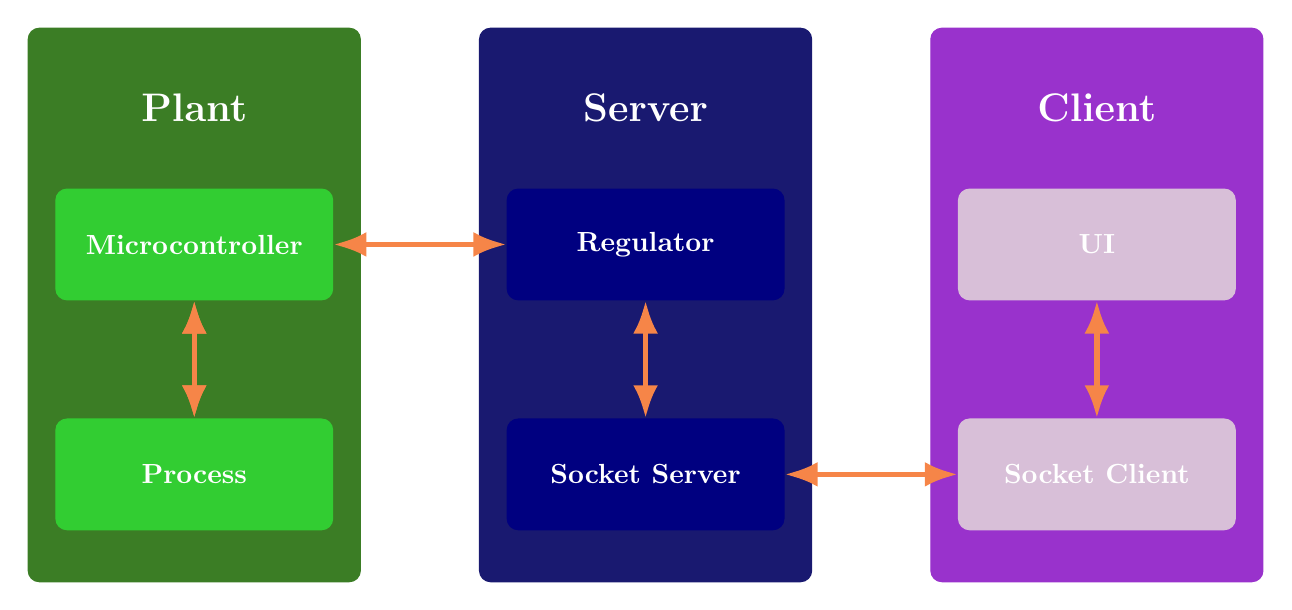
\begin{tikzpicture}
    \node[draw=OliveGreen, rectangle, minimum width=120, minimum height=200,
    label={[label distance=-180, font=\Large\bf, color=white]-90:Plant},
    fill=OliveGreen, rounded corners]
    (plant) {};

    \node[draw=MidnightBlue, rectangle, minimum width=120, minimum height=200,
    label={[label distance=-180, font=\Large\bf, color=white]-90:Server},
    fill=MidnightBlue, rounded corners, right=1.5 of plant]
    (daemon) {};

    \node[draw=DarkOrchid, rectangle, minimum width=120, minimum height=200,
    label={[label distance=-180, font=\Large\bf, color=white]-90:Client},
    fill=DarkOrchid, rounded corners, right=1.5 of daemon]
    (client) {};

    \node[draw=LimeGreen, rectangle, rounded corners, minimum height=40,
          minimum width=100, fill=LimeGreen, below=-5 of plant, font=\bf]
          (arduino) {\textcolor{white}{Microcontroller}};

    \node[draw=LimeGreen, rectangle, rounded corners, minimum height=40,
          minimum width=100, fill=LimeGreen, below=1.5 of arduino, font=\bf]
          (process) {\textcolor{white}{Process}};

    \node[draw=NavyBlue, rectangle, rounded corners, minimum height=40,
          minimum width=100, fill=NavyBlue, below=-5 of daemon, font=\bf]
          (regulator) {\textcolor{white}{Regulator}};

    \node[draw=NavyBlue, rectangle, rounded corners, minimum height=40,
          minimum width=100, fill=NavyBlue, below=1.5 of regulator, font=\bf]
          (sserver) {\textcolor{white}{Socket Server}};

    \node[draw=Thistle, rectangle, rounded corners, minimum height=40,
          minimum width=100, fill=Thistle, below=-5 of client, font=\bf]
          (UI) {\textcolor{white}{UI}};

    \node[draw=Thistle, rectangle, rounded corners, minimum height=40,
          minimum width=100, fill=Thistle, below=1.5 of UI, font=\bf]
          (sclient) {\textcolor{white}{Socket Client}};

    \draw[Latex-Latex, line width=2, color=Peach] (arduino) to (regulator);
    \draw[Latex-Latex, line width=2, color=Peach] (arduino) to (process);
    \draw[Latex-Latex, line width=2, color=Peach] (arduino) to (process);
    \draw[Latex-Latex, line width=2, color=Peach] (sserver) to (sclient);
    \draw[Latex-Latex, line width=2, color=Peach] (regulator) to (sserver);
    \draw[Latex-Latex, line width=2, color=Peach] (UI) to (sclient);
\end{tikzpicture}
\caption{Shematski prikaz rada}
\label{fig:main_sheme}
\end{figure}

Na slici \ref{fig:main_sheme} je prikazan sinopsis diplomskoga rada koji je podijeljen u 3 dijela:
\begin{itemize}
        \item Postrojenje
        \item Server
        \item Klijent
\end{itemize}

Kao što je već spomenuto u poglavlju \ref{introduction}, postrojenje se sastoji
od mikroupravljača i dviju boca koje služe kao model za održavanje razine vode.

Server, koji je pisan u Haskellu, također se sastoji od dva dijela, regulatora i
socket servera. Regulacijski dio s postrojenjem komunicira pomoću Firmata
protokola, a socket server s klijentima komunicira pomoću JSON-RPC protokola.

Klijent koji je pisan u Pythonu sastoji se od korisničkog sučelja i socket
klijenta koji periodički dohvaća trenutno stanje postrojenja od servera.

\section{Haskell}

Haskell je moderan, standardan, nije striktan, čisto funkcionalan programski
jezik. Dizajniran je za širok spektar primjena, od numeričkih do
simboličkih \cite{haskell_intro}.

Haskell je nastao 1990. godine te nakon nekoliko godina razvoja glavne osobine
bile su mu \cite{haskell_history}:

\begin{itemize}
\item Statički pisan
\item Sigurnost tipova
\item Lijenost
\item Klase tipova.
\end{itemize}

Statički pisan jezik zahtijeva da pri kompilaciji koda svi tipovi podataka budu
poznati, što donosi niz prednosti kao primjećivanje grešaka prije nego što se
program izvrši, efikasniji kod jer compiler zna unaprijed veličinu podataka,
nije potrebno provjeravati tip podatka dok se program izvršava.

Sigurnost tipova proizlazi iz strogo statičkog pisanja. Ona osigurava
funkcije od primanja podatak pogrešnog tipa. Takve će greške prepoznati compiler pri
kompilaciji.

Lijenost (engl. \emph{Lazy evaluation}) je svojstvo jezika pri kojem se izrazi
evaluiraju tek kada je to potrebno. Rezultat komputacije računa se tek kada je
on zatražen negdje dalje. Lazy evaluation omogućuje elegantan rad s beskonačnim
poljima. Moguće je definirati polje s beskonačnim brojem članova, a da program
ne zauzme svu memoriju računala. Pojedini će se elementi polja evaluirati ako, i
samo ako, mu probamo pristupiti.

Klase tipova (engl. \emph{Type classes}) nastale kako bi omogućile
implementiranje preopterećenih aritmetičkih operatora i operatora jednakosti.

\subsection{Mrežno programiranje}
\label{subsect:haskell_net}

Za mrežno programiranje Haskell nudi modul
\mintinline{haskell}{Network.Socket} \cite{network_socket}, koji korisniku
pruža sve standardne C funkcije za stvaranje UNIX socketa.

\begin{figure}[H]
\centering

\begin{tikzpicture}[every node/.style = {font=\large\bf, rectangle,
                    rounded corners, minimum width=70},
                    connection/.style = {-Latex, Peach, line width=2}]
    \node[draw=OliveGreen, fill=OliveGreen]
          (socket) {\textcolor{white}{socket()}};

    \node[draw=MidnightBlue, fill=MidnightBlue, right=of socket]
          (bind) {\textcolor{white}{bind()}};

    \node[draw=Sepia, fill=Sepia, right=of bind]
          (listen) {\textcolor{white}{listen()}};

    \node[draw=DarkOrchid, fill=DarkOrchid, right=of listen]
          (accept) {\textcolor{white}{accept()}};

    \draw[connection] (socket) to (bind);
    \draw[connection] (bind)   to (listen);
    \draw[connection] (listen) to (accept);
\end{tikzpicture}
\caption{Programski tok izrade socket servera}
\label{fig:server_creation}
\end{figure}

Na slici \ref{fig:server_creation} je prikazan programski slijed izrade
socket servera. Prvo se pomoću \mintinline{haskell}{socket} funckcije stvori
socket određenih karakteristika. U \mintinline{haskell}{Network.Socket} modulu
je funkcija definirana kao:
\mint{haskell}|socket :: Family -> SocketType -> ProtocolNumber -> IO Socket|

Iz definicije funkcije vidljivo je kako je ona zapravo ista kao i standardna C
funkcija za stvaranje socketa \cite[str.132]{unixnetwork}. Nakon što je stvoren
socket njemu se treba dodijeliti lokalna adresa odabranog protokola,
dodjeljivanje adrese postiže se s \mintinline{haskell}{bind} funkcijom čija
definicija glasi:
\mint{haskell}|bind :: Socket -> SockAddr -> IO ()|

Slijedi pretvaranje stvorenog socketa u pasivni socket koji će čekati na ulazne
konekcije. To se ostvaruje pomoću funkcije \mintinline{haskell}{listen} koja je
definirana kao:
\mint{haskell}|listen :: Socket -> Int -> IO ()|

Na kraju je još potrebno pričekati konekciju klijenta što se ostvaruje s
funkcijom \mintinline{haskell}{accept} koja blokira daljni tok programa dok se
klijent ne spoji. Definicija funkcije glasi:
\mint{haskell}|accept :: Socket -> IO (Socket, SockAddr)|
Funkcija nam vraća novi socket s pomoću kojim možemo razmjenjivati podatke s
klijentom i adresu klijenta. Razmjena se podataka može vršiti s
\mintinline{haskell}{sendTo} i \mintinline{haskell}{recvFrom} no radi
jednostavnosti možemo socket pretvoriti u handle te pisati i čitati podatke
kao da se radi o datoteci. Za to postoji \mintinline{haskell}{socketToHandle}
koja jednostavno primi socket i mode u kojem treba biti handle (read, write ili
oboje) i vrati handle. Definicija joj glasi:
\mint{haskell}|socketToHandle :: Socket -> IOMode -> IO Handle|

\subsection{Istodobnost}

Istodobnost (engl. \emph{Concurrency}) je svojstvo sustava kojim se istodobno
može izvršavati više računskih operacija ili komputacija.

Ekstenzija za istodobnost u Haskellu pojavila se 1996. godine koja uvodi dva
nova idioma u Haskell \cite{concurrent}:
\begin{itemize}
        \item Procese i mehanizme za stvaranje procesa
        \item Atomarno promjenjivo stanje
\end{itemize}

Istodobnost u Haskellu uglavnom je izvedena pomoću "Zelenih niti"
(engl.\emph{Green threads}). Zelene niti ne izvršavaju se u jezgri operativnog
sustava već u \emph{Haskell runtime-u}. Haskell ima hibridni višenitni
model kojim se N Haskell niti mogu vezivati na M niti operativnog sustava.

\begin{figure}[H]
\centering
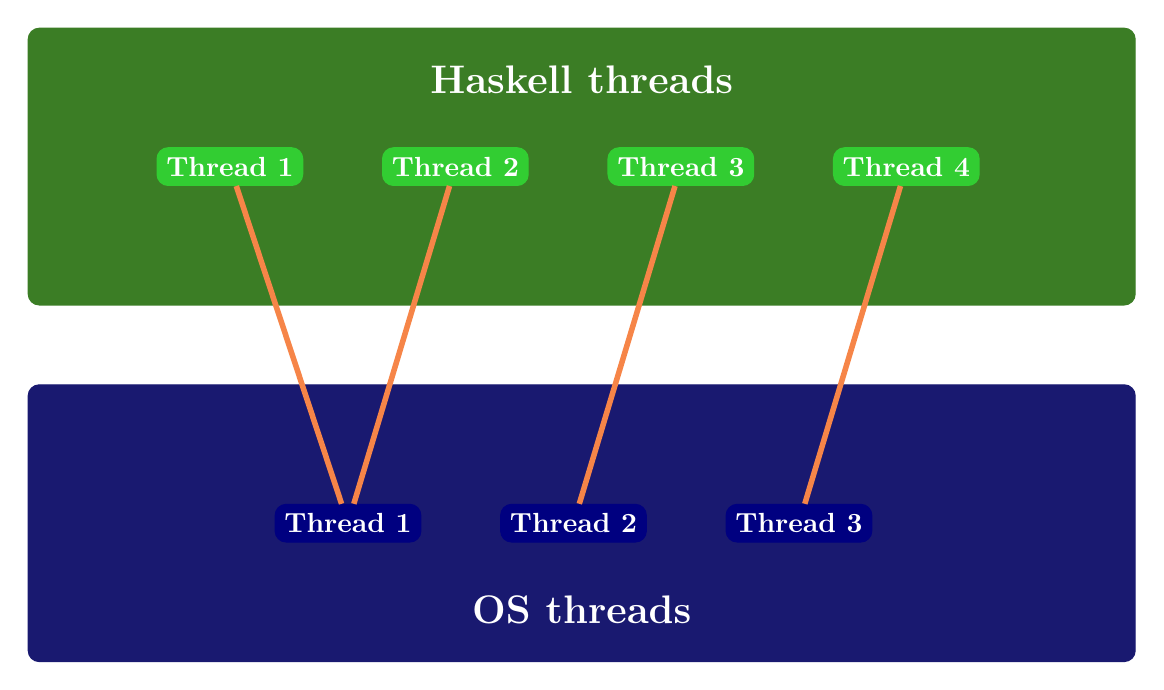
\begin{tikzpicture}
    \node[draw=OliveGreen, rectangle, minimum width=400, minimum height=100,
    label={[label distance=-90, font=\Large\bf, color=white]-90:Haskell threads},
    fill=OliveGreen, rounded corners]
    (hThreads) {};

    \node[draw=LimeGreen, rectangle, rounded corners,
          fill=LimeGreen, left=-3.5 of hThreads, font=\bf]
          (hThread1) {\textcolor{white}{Thread 1}};

    \foreach [count=\j from 1] \i in {2,...,4} {
        \node[draw=LimeGreen, rectangle, rounded corners,
              fill=LimeGreen, font=\bf, right=of hThread\j]
              (hThread\i) {\textcolor{white}{Thread \i}};
    }

    \node[draw=MidnightBlue, rectangle, rounded corners, minimum width=400,
          minimum height=100, below=of hThreads, label={[label distance=-90,
          font=\Large\bf, color=white]90:OS threads}, fill=MidnightBlue]
          (osThreads) {};

    \node[draw=NavyBlue, fill=NavyBlue, rectangle, rounded corners,
          left=-5.0 of osThreads, font=\bf] (osThread1)
          {\textcolor{white}{Thread 1}};

    \foreach [count=\j from 1] \i in {2,...,3} {
        \node[draw=NavyBlue, fill=NavyBlue, font=\bf, rectangle,
              rounded corners, right=of osThread\j]
              (osThread\i) {\textcolor{white}{Thread \i}};
    }

    \draw[line width=2, color=Peach] (hThread1) to (osThread1);
    \draw[line width=2, color=Peach] (hThread2) to (osThread1);
    \draw[line width=2, color=Peach] (hThread3) to (osThread2);
    \draw[line width=2, color=Peach] (hThread4) to (osThread3);
\end{tikzpicture}
\caption{N:M višenitni model Haskell-a}
\label{fig:thread_model}
\end{figure}

Na slici \ref{fig:thread_model} je prikazano kako se Haskell niti mapiraju na
niti operativnog sustava.
Interno se u Haskellu stvaranje nove niti pretvara u alokaciju strukture koja
sprema trenutno stanje niti te se niti pretvaraju u jednu petlju.

Za stvaranje nove niti Haskell nudi \mintinline{haskell}{forkIO} funkciju koja
je dio \mintinline{haskell}{Control.Concurrent} modula
\cite{control_concurrent}, a definirana je kao:
\mint{haskell}|forkIO :: IO () -> IO ThreadId|

Što znači da funkcija kao prvi argument prima komputaciju (engl.
\emph{computation}) i vraća novu komputaciju koja kao rezultat proizvodi
\mintinline{haskell}{ThreadId}, što nam služi kao referenca na novu nit koju će
funkcija stvoriti.

Osim niti za istodobno izvršavanje programa, bitna je i komunikacija između niti.
Za komunikaciju između niti Haskell nudi mutabilne dijeljene varijable zvane
\mintinline{haskell}{MVar} (Mutable Variables) koje se nalaze unutar
\mintinline{haskell}{Control.Concurrent.MVar} modula \cite{mvar}. One se mogu
koristiti na razne načine:

\begin{itemize}
\item Sinkronizirane mutabilne varijable.
\item Komunikacijski kanali između niti.
\item Binarni semafori.
\end{itemize}

Nova mutabilna varijabla koja sadrži podatak proizvoljnog tipa može se napraviti
s \mintinline{haskell}{newMVar}, definirana je kao:
\mint{haskell}|newMVar :: a -> IO (MVar a)|

Nakon što je varijabla stvorena, njom se može na razne načine manipulirati, između
ostalog može se zapisati novi podatak u nju, pročitati podatak ili zamijeniti s
nekim drugim podatkom.

Čitanje podatka bez njegove izmjene omogućuje nam
\mintinline{haskell}{readMVar}:
\mint{haskell}|readMVar :: MVar a -> IO a|

Za zamjenu podatka s nekim drugim postoji \mintinline{haskell}{swapMVar}
funkcija:
\mint{haskell}|swapMVar :: MVar a -> a -> IO a|

Za izmjenu više dijeljenih varijabli postoji
\mintinline{haskell}{Control.Concurrent.Chan} \cite{conc.chan} modul, koji
sadržava implementaciju neograničenog komunikacijskog kanala.

Novi komunikacijski kanal stvara se s \mintinline{haskell}{newChan} funkcijom:
\mint{haskell}|newChan :: IO (Chan a)|

Funkcija stvara novi prazni komunikacijski kanal određenog tipa te ga vraća kao
rezultat. Komunikacijski sprema vrijednosti i čuva ih sve dok ih se ne izvadi iz
njega. Služi kao FIFO spremnik vrijednosti određenog tipa.

Novi podatak stavlja se u kanal \mintinline{haskell}{writeChan}
funkcijom:
\mint{haskell}|writeChan :: Chan a -> a -> IO ()|

Funkcija kao argument prima komunikacijski kanal i podatak. Tip podatka mora
odgovarati tipu podatka određenog pri stvaranju komunikacijskog kanala.
Vrijednost se sprema u kanal te tamo ostaje sve dok se ona ne pročita
\mintinline{haskell}{readChan} funkcijom:
\mint{haskell}|readChan :: Chan a -> IO a|

\mintinline{haskell}{readChan} funkcija kao argument prima komunikacijski kanal
i vraća najstariji podatak koji se nalazi u kanalu.

\newpage
\section{Python}

Python je interpretiran, objektno orijentiran, programski jezik visoke razine
s dinamičkom semantikom. Podatkovne strukture visoke razine i dinamičko pisanje
čine ga atraktivnim za vrlo brzo razvijanje aplikacija i za skriptni jezik za
spajanje više postojećih komponenti.
Python posjeduje jednostavnu i laku sintaksu koja povećava čitljivost i
olakšava održavanje softver-a \cite{python_ref}.

\subsection{Mrežno programiranje}

Slično kao i Haskell, Python pruža sve standardne C funkcije za mrežno
programiranje. Sve se bitne funkcije nalaze u \mintinline{python}{Socket}
modulu \cite{python_socket}.

\begin{figure}[H]
\centering

\begin{tikzpicture}[every node/.style = {font=\large\bf, rectangle,
                    rounded corners, minimum width=80},
                    connection/.style = {-Latex, Peach, line width=2}]
    \node[draw=OliveGreen, fill=OliveGreen]
          (socket) {\textcolor{white}{socket()}};

    \node[draw=DarkOrchid, fill=DarkOrchid, right=of socket]
          (connect) {\textcolor{white}{connect()}};

    \draw[connection] (socket) to (connect);
\end{tikzpicture}
\caption{Programski tok izrade socket klijenta}
\label{fig:client_creation}
\end{figure}

Na slici \ref{fig:client_creation} je prikazan programski tok izrade socket
klijenta. Slično kao i sa serverom, prvo se stvori socket:
\mint{python}|socket.socket()|

Socket mora biti iste vrste kao i socket servera na koji se želimo spojiti.
Nakon stvaranja socketa potrebno ga je spojiti na serverski kraj socketa.
Spajanje na server vrši se pomoću \mintinline{py3}{connect()} funkcije kojoj se
predaje adresa i port socket servera:
\mint{python}|socket.connect()|

Nakon spajanja može započeti komunikacija između klijenta i servera.
Komunikacija se može izvršiti pomoću standardnih C funkcija \mintinline{c}{send}
i \mintinline{c}{recv} ili, kao i u Haskellu, socket se može pretvoriti u handle
te se koristiti kao da je datoteka:
\mint{python}|socket.makefile()|

Izrada socket-klijenta daleko je lakša od servera, pogotovo jer se nerijetko ne
moramo brinuti o više istovremenih konekcija.

\newpage
\subsection{Urwid}

Urwid je Python biblioteka za izradu tekstualnih korisničkih sučelja. Urwid je
alternativa za standardnu Curses biblioteku \cite{curses}. Interno
koristi Curses biblioteku, no Urwid olakšava neke teže poslove pri izradi
tekstualnih sučelja \cite{urwid}.

Programi s Curses tekstualnim sučeljem često sliče programima s grafičkim
sučeljem koji posjeduju tekstualne kutije, razne forme za ispunjavanje, liste
s navigacijskim trakama i gumbe. Takvi grafički elementi olakšavaju korištenje 
programa, naspram standardnih tekstualnih programa, a ujedno omogućavaju rad na
na čisto tekstualnim uređajima. Programi s Curses tekstualnim sučeljem
također zahtijevaju manje resursa naspram grafičkih programa.

Urwid koristi događajnu petlju (engl. \emph{Event loop}) koja olakšava
rukovanje programskim ulazima i osvježavanje sučelja.

\subsection{Event loop}

Event loop je programski konstrukt koji čeka i otprema događaje ili poruke
unutar programa. Event loop šalje zahtjev pružatelju događaja (koji uglavnom
blokira sve dok neki događaj ne bude dostupan) te zatim poziva određenog
rukovatelja. Event loop je jedan od načina asinkronog programiranja.

\begin{figure}[H]
\centering
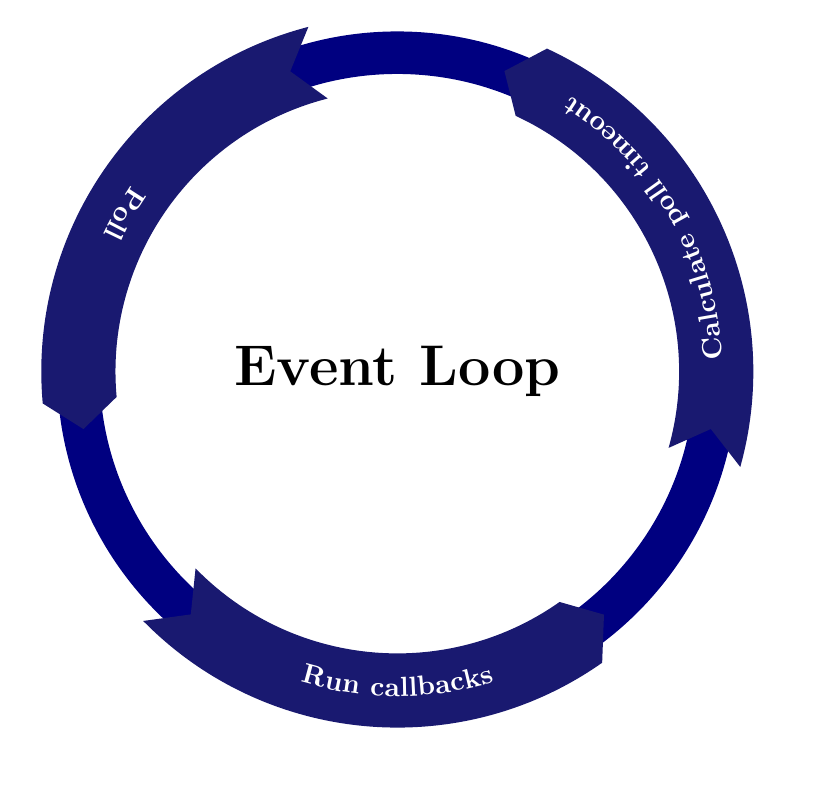
\begin{tikzpicture}[scale=0.9]
\newcommand{\arcarrow}[8]% inner radius, middle radius, outer radius, start angle, end angle, tip protusion angle, options, text
{   \pgfmathsetmacro{\rin}{#1}
    \pgfmathsetmacro{\rmid}{#2}
    \pgfmathsetmacro{\rout}{#3}
    \pgfmathsetmacro{\astart}{#4}
    \pgfmathsetmacro{\aend}{#5}
    \pgfmathsetmacro{\atip}{#6}
    \fill[#7] (\astart:\rin) arc (\astart:\aend:\rin) -- (\aend+\atip:\rmid) -- (\aend:\rout) arc (\aend:\astart:\rout) -- (\astart+\atip:\rmid) -- cycle;
    \path[decoration={text along path, text={|\color{white}\bf|#8}, text align={align=center}, raise=-0.5ex},decorate] (\astart+\atip:\rmid) arc (\astart+\atip:\aend+\atip:\rmid);
}

    \fill[even odd rule,NavyBlue] circle (4.8) circle (4.2);
    \draw (0, 0) node {\huge \bf Event Loop};

    \arcarrow {4}{4.5}{5}{325+20}{325+100}{5} {fill=MidnightBlue,
                draw=MidnightBlue, very thick} {Calculate poll timeout};
    \arcarrow {4}{4.5}{5}{85+20}{85+100}{5} {fill=MidnightBlue,
                draw=MidnightBlue, very thick} {Poll};
    \arcarrow {4}{4.5}{5}{205+20}{205+100}{5} {fill=MidnightBlue,
                draw=MidnightBlue, very thick} {Run callbacks};
\end{tikzpicture}
\caption{Programski tok \emph{Event loopa}}
\label{fig:event_loop}
\end{figure}

Na slici \ref{fig:event_loop} je prikazan programski tok Event loop-a. Prvo se
izračuna koliko će se čekati na događaj, pa se pomoću Unix sistemskog poziva
\emph{poll} čeka na događaj te se na kraju poziva funkcija koja je namijenjena za
obradu određenog događaja.

\newpage
\section{Arduino}

Arduino je mali uređaj za izradu računalnih sustava koji mogu mjeriti fizikalne
veličine i upravljati fizičkim svijetom. Arduino je open-source računalni sustav
koji se temelji na jednostavnoj mikroupravljačkoj pločici i razvojnom okruženju za
pisanje softvera.

Arduino se može koristiti za razvoj interaktivnih fizičkih objekata, može
primati ulazne fizikalne veličine od raznih senzora i upravljati sa svijetlima,
motorima ili drugim fizičkim izlazima. Arduino projekti mogu biti samostalni ili
mogu komunicirati sa softverom koji se nalazi na računalu.
\cite{arduino_intro}.

\begin{figure}[H]
\centering
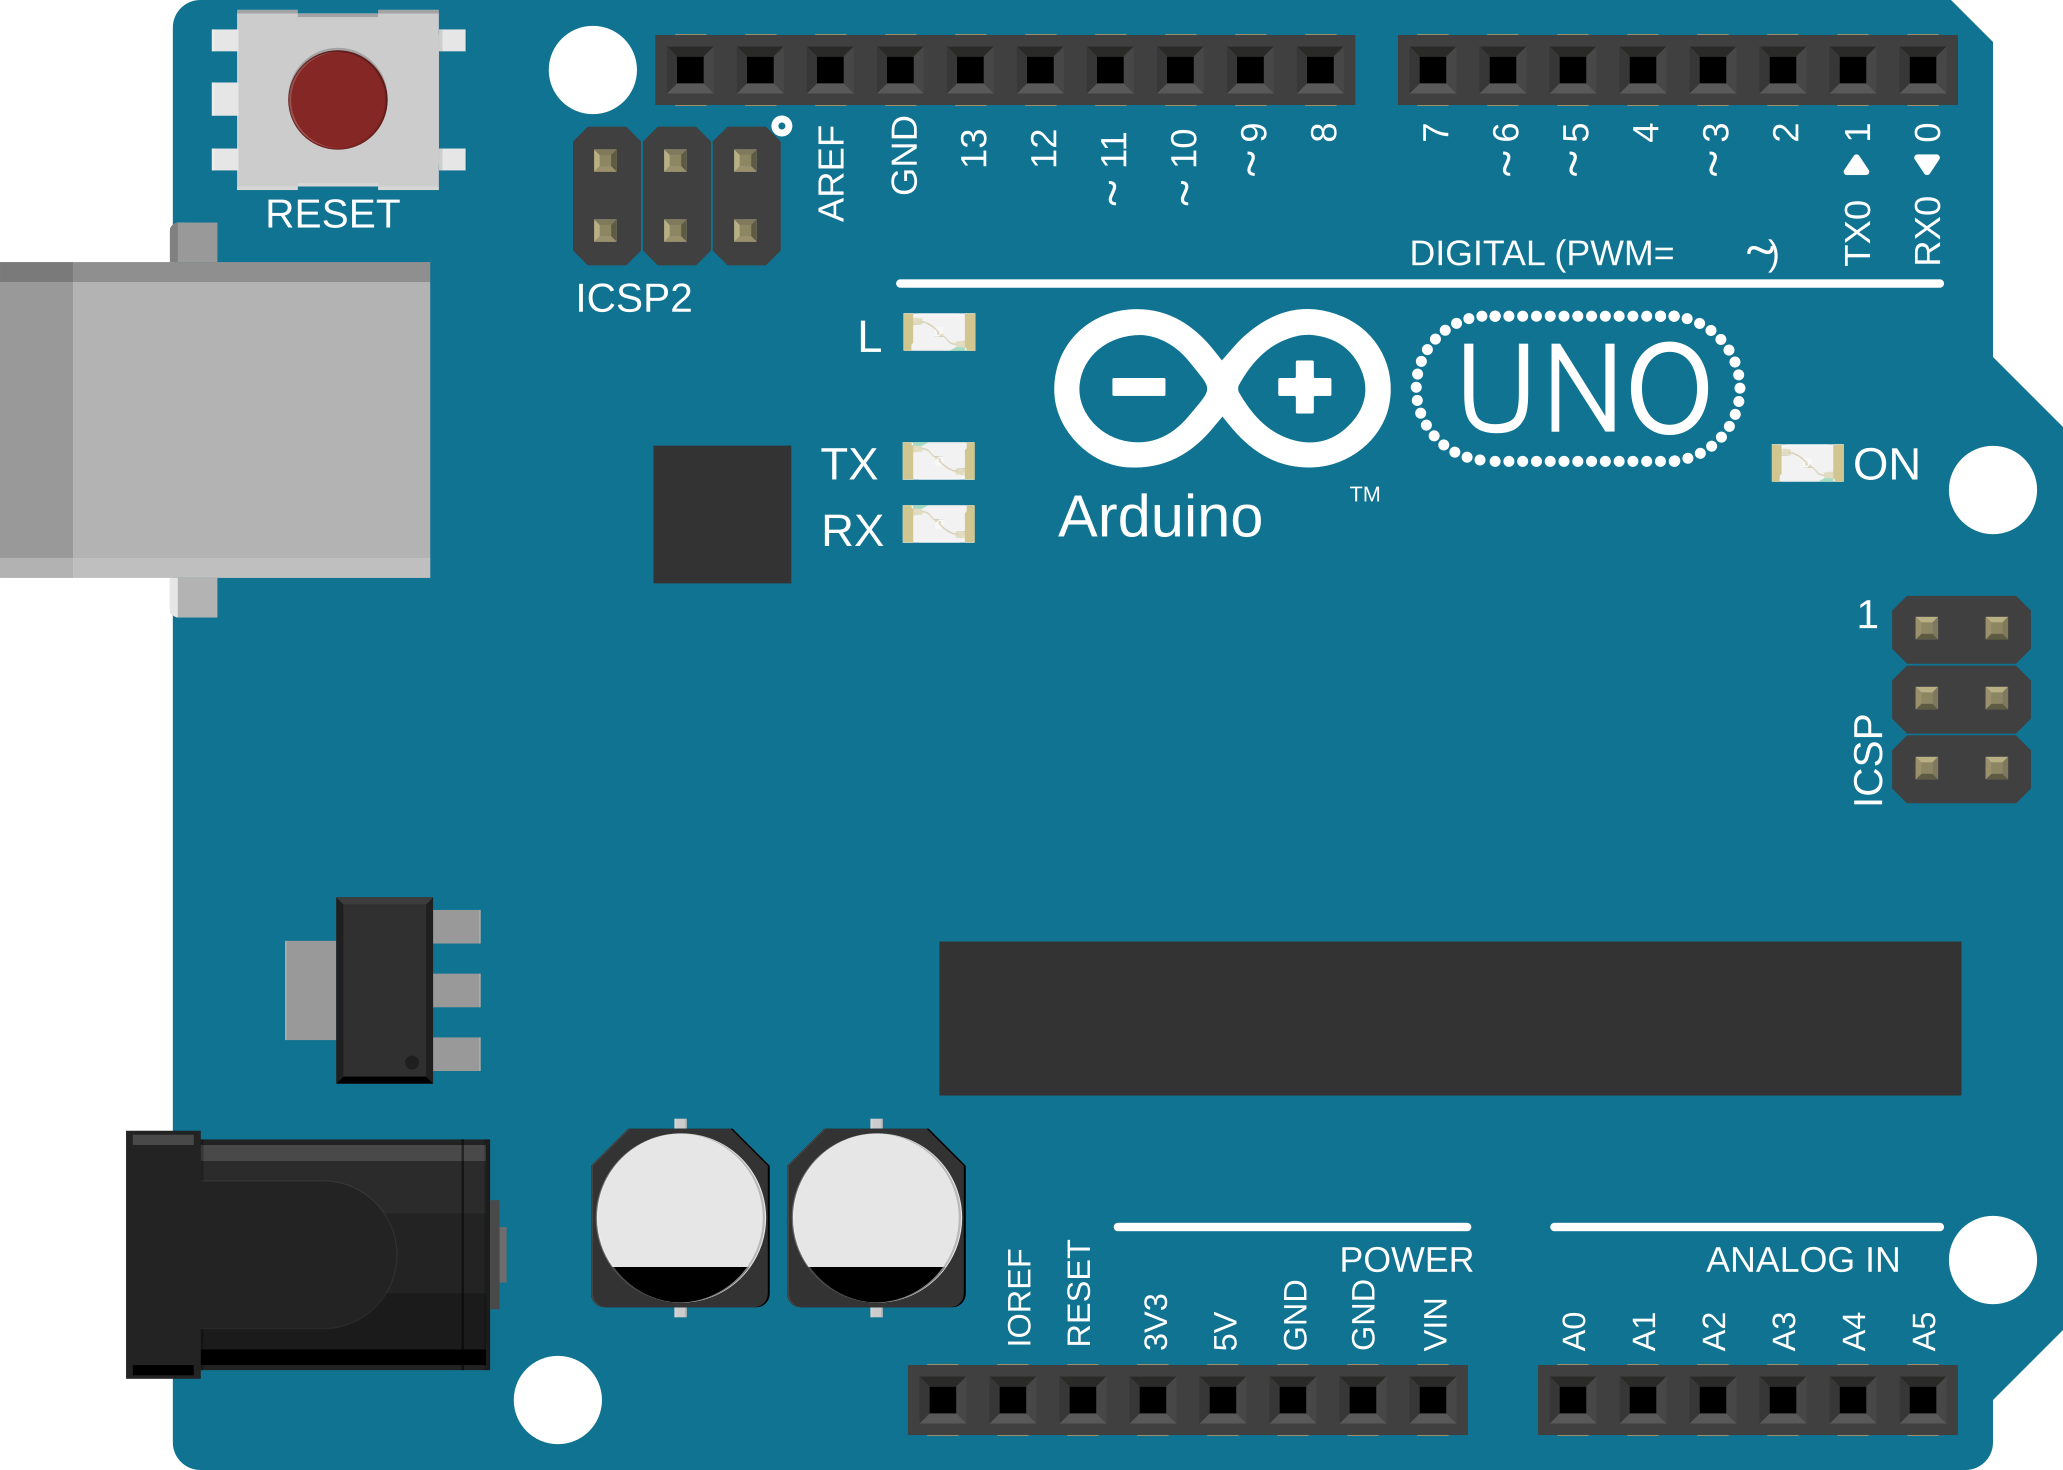
\includegraphics[scale=1.6]{figures/arduino_uno.pdf}
\caption{Arduino UNO mikroupravljačka ploča.\protect\footnotemark}
\label{fig:arduino}
\end{figure}

\footnotetext{Izvorna slika, licencirana pod Creative Commons
    Attribution-ShareALike 3.0 preuzeta je i prilagođena od Fritzing projekta
(\url{https://raw.githubusercontent.com/fritzing/fritzing-parts/master/svg/core/breadboard/arduino_Uno_Rev3_breadboard.svg})}

Na slici \ref{fig:arduino} se vidi Arduino UNO mikroupravljačka ploča. Kao
mikroupravljač koristi se ATmega328 \cite{atmega}. Mikroupravljačka pločica posjeduje 14
digitalnih ulazno/izlaznih pinova, od kojih se 6 mogu koristiti kao pulsno
širinski modulirani izlazi, 6 analognih ulaza, \unit{16}{\mega\hertz} keramički
oscilator, USB sučelje, ulaz za eksterno napajanje i reset tipku. Pločica se
može napajati preko USB sučelja ili preko ulaza za eksterno napajanje.
Komunikacija s računalom odvija se preko USB-serijskog sučelja. Za programski
dio mikroupravljač sadrži \unit{32}{\kilo\byte} flash memorije koje se mogu programirati.

\newpage
\section{Firmata}

Firmata je jednostavan protokol baziran na MIDI-ju i koji je namijenjen za komunikaciju
računala s mikroupravljačem. Cilj mu je omogućiti direktno upravljanje što većim
dijelom mikroupravljača od strane računala.

Za podatkovni format protokola odabrane su MIDI \cite{midi} poruke. Nije u
potpunosti kompatibilan s MIDI standardom, budući da se koristi brža serijska
konekcija i poruke se ne preklapaju u svim slučajevima. No za parsiranje poruka
moguće je koristiti postojeće MIDI parsere.

Protokol se može implementirati kao firmware za bilo koji mikroupravljač ili kao
softver za računalo. Firmata je prvi puta implementirana za mikroupravljače za
Arduino obitelj mikroupravljača. Kao računalni softver, postoji mnogo Firmata 
implementacija za razne jezike, između ostalog i za Python \cite{pyfirmata}
i Haskell \cite{harduino}

\begin{table}[h]
\setlength{\tabcolsep}{18pt}
\centering
    \begin{tabular}{|c|c|}
        \hline
        Naredba               & Numerička vrijednost \\
        \hline
        analog I/O message    & 0xE0 \\
        \hline
        digital I/O message   & 0x90 \\
        \hline
        report analog pin     & 0xC0 \\
        \hline
        report digital port   & 0xD0 \\
        \hline
        start sysex           & 0xF0 \\
        \hline
        set pin mode(I/O)     & 0xF4 \\
        \hline
        set digital pin value & 0xF5 \\
        \hline
        sysex end             & 0xF7 \\
        \hline
        protocol version      & 0xF9 \\
        \hline
        system reset          & 0xFF \\
        \hline
    \end{tabular}
    \caption{Firmata naredbe}
    \label{tbl:firmata}
\end{table}

Na tablici \ref{tbl:firmata} se vide neke od Firmata naredbi i njihove
odgovarajuće numeričke vrijednosti. Da bi se naredio reset mikroupravljača,
jednostavno se preko serijske veze pošalje vrijednost 0xFF te, nakon što
mikroupravljač primi poruku, izvršit će reset rutinu.

\newpage
\section{JSON-RPC}

JSON-RPC je jednostavan protokol za udaljene proceduralne pozive, ne sadržava
stanje i nije definiran kao transportni protokol \cite{jsonRPC}. Koristi JSON
\cite{jsonRFC} kao podatkovni format.

Pozivna poruka sastoji se od:
\begin{itemize}
        \item jsonrpc - verzija protokola
        \item method - ime udaljene metode koja se poziva
        \item params - ulazni parametri za metodu
        \item id - identifikacijska oznaka poruke
\end{itemize}

Ulazni parametri moraju biti strukturiran podatak. Mogu biti u obliku niza ili
JSON objekta, s imenovanim varijablama koje odgovaraju parametrima pozvane
metode.

Odgovor se sastoji od:
\begin{itemize}
    \item jsonrpc - verzija protokola ("2.0")
    \item result - rezultat koji vraća pozvana metoda
    \item error - greška ako ona postoji
    \item id - identifikacijska oznaka poruke
\end{itemize}

Ako dolazi do greške odgovor neće sadržavati rezultat, nego će rezultat će
zamijeniti greška, a svi ostali dijelovi odgovora ostaju isti.
Identifikacijska oznaka u odgovoru mora biti ista kao i u pozivu.

Primjer poziva:
\mint{json}|{"jsonrpc": "2.0", "method": "subtract", "params": [42, 23], "id": 1}|

Tu se vidi poziv koji koristi verziju 2.0 JSON-RPC protokola. Ona poziva metodu
\emph{substract} kojoj predaje parametre u obliku niza (brojčane vrijednosti 42
i 23) te koristi identifikacijsku oznaku s brojem 1.

Primjer odgovora za prethodnu pozivnu poruku:
\mint{json}|{"jsonrpc": "2.0", "result": 19, "id": 1}|

U odgovoru je vidljivo kako server koristi isti protokol kao i klijent, vraća rezultat
pozvane metode te koristi istu identifikacijsku oznaku kao što je dobio u
pozivnoj poruci od klijenta.


\newpage
\chapter{Implementacija}

U ovom poglavlju je objašnjena implementacija socket servera, odgovarajućeg
klijenta i na kraju samog postrojenja.
Detaljno je opisana arhitektura servera, klijenta te izrada makete postrojenja.

\section{Server}

Server je centralni dio rada. Na slici \ref{fig:main_sheme} u poglavlju
\ref{chpt:first} se vidi njegova uloga. Komunicira s postrojenjem s jedne strane
i s klijentima s druge strane. Dizajn servera se oslanja na istodobnost i
modularnost.

Glavni poslovi servera su jasno razdvojeni u različite niti. Server
sadržava tri glavne niti od koje se jedna brine oko regulacije postrojenja,
jedna prihvaćanju konekcija klijenta i jedna kao posrednička nit između
klijenata i regulacijske niti. Nit koja se brine oko prihvaćanju konekcija od
strane klijenta za svakog klijenta stvara novu nit te se prihvaćanje novih
konekcija nesmetano može nastaviti.

\begin{figure}[H]
\centering
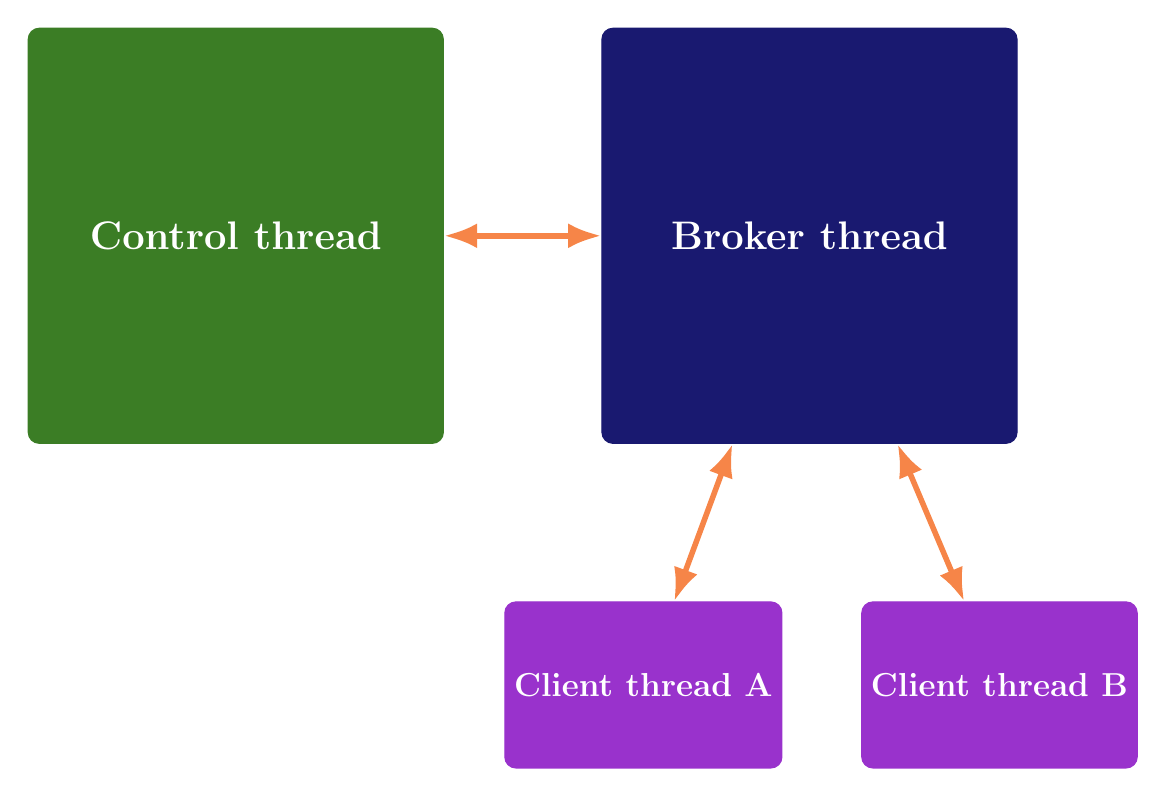
\begin{tikzpicture}[every node/.style = {font=\Large\bf},
                    connection/.style = {Latex-Latex, Peach, line width=2}]
    \node[draw=OliveGreen,rectangle, rounded corners,
          fill=OliveGreen, minimum size=150]
          (regulator) {\textcolor{white}{Control thread}};

    \node[draw=MidnightBlue, rectangle, rounded corners, minimum size=150,
          right=2cm of regulator, fill=MidnightBlue]
          (server) {\textcolor{white}{Broker thread}};

    \node[draw=DarkOrchid, rectangle, rounded corners,
          minimum size=60, below left=2cm and -2.3cm of server, font=\bf\large,
          fill=DarkOrchid]
          (clientA) {\textcolor{white}{Client thread A}};

    \node[draw=DarkOrchid, rectangle, rounded corners,
          minimum size=60, right=of clientA, font=\bf\large,
          fill=DarkOrchid]
          (clientB) {\textcolor{white}{Client thread B}};

    \draw[connection] (regulator) to (server);
    \draw[connection] (server)    to (clientA);
    \draw[connection] (server)    to (clientB);
\end{tikzpicture}
\caption{Arhitektura servera}
\label{fig:architecture}
\end{figure}

Na slici \ref{fig:architecture} je prikazana komunikacija između pojedinih niti
unutar servera. Regulacijska nit označena zelenom bojom čita referentnu
vrijednost iz djeljene varijable koju postavlja posrednička nit, označena plavom
bojom, a postavlja mjerenu procesnu veličinu u drugu dijeljenu varijablu koje
klijentske niti mogu direktno očitati. Zbog zahtjeva za atomarnosti operacija
čitanja i pisanja dijeljenih varijabli nije moguće odobriti više od jednoj niti
zapisivanje u pojedinu dijeljenu varijablu, te radi toga postoji posrednička nit
koja od raznih klijentskih niti preuzima referentnu vrijednost i atomarno
prosljeđuje regulacijskoj niti.

\begin{listing}[H]
\centering
\begin{minted}[frame=single]{haskell}
startDaemon :: Integer -> FilePath -> Bool -> IO ()
startDaemon port arduinoPort simulate = do
    sock <- socket AF_INET Stream 0

    bindSocket sock $ SockAddrInet (fromInteger port) iNADDR_ANY
    listen sock 50

    pv <- newMVar 0
    referenceChan <- newChan
    let com = ProcCom pv referenceChan

    _ <- forkIO $ serverLoop sock com

    controllerBroker arduinoPort simulate com
\end{minted}
\caption{Main entry point}
\label{lst:main}
\end{listing}

Na ispisu koda \ref{lst:main} je prikazana glavna funkcija, zvana
\mintinline{haskell}{startDaemon}, koja pokreće server.
Funkcija prolazi skoro kroz sve korake koji su prikazani na slici
\ref{fig:server_creation} u poglavlju \ref{subsect:haskell_net}, prvo stvara
socket, te ga povezuje s lokalnom adresom i portom. Nakon toga se socket
pretvara u pasivni socket koji prihvaća maksimalno 50 konekcija. Nakon stvaranja
socketa i njegove pripreme stvara se jedna dijeljena varijabla te jedan
komunikacijski kanal.

Dijeljena varijabla će sadržavati mjerenu procesnu veličinu, to jest razinu vode
u spremniku, dok će se komunikacijski kanal puniti sa željenim referentnim
veličinama od strane klijenata. Kako pojedina referentna veličina stigne od
strane klijenta ona se stavlja u komunikacijski kanal te će ih kasnije
posrednička nit vaditi iz komunikacijskog kanala te proslijediti
regulacijskoj niti.

Na kraju se logika za socket server odvaja u novu nit sa
\mintinline{haskell}{forkIO} funkcijom koja kao argument prima
\mintinline{haskell}{serverLoop} funkciju i njene argumente. Glavna nit poziva
\mintinline{haskell}{controllerBroker} funkciju koja će nastavit sa pripremom
regulacijske niti.

\begin{listing}[H]
\centering
\begin{minted}[frame=single]{haskell}
serverLoop :: Socket -> ProcCom PVType -> IO ()
serverLoop sock com = do
    (s, host) <- accept sock
    let hostinfo = show host
    noticeM rootLoggerName $ "Connected:    " ++ hostinfo
    hdl <- socketToHandle s ReadWriteMode
    _ <- forkIO $ runConn hdl com hostinfo

    serverLoop sock com
\end{minted}
\caption{Server mainloop}
\label{lst:serverLoop}
\end{listing}

Na ispisu koda \ref{lst:serverLoop} se vidi \mintinline{haskell}{serverLoop}
funkcija, ona sa funkcijom \mintinline{haskell}{accept} čeka na konekciju
klijenta, funkcija blokira sve dok se klijent ne spoji.

Za svakog klijenta koji se spoji na server ispisuje se informacija o klijentu,
pretvara se socket u handle sa \mintinline{haskell}{socketToHandle} funkcijom,
te se stvara nova nit koja će izvržavati \mintinline{haskell}{runConn} funkciju,
ona je zadužena za komunikaciju s klijentom te će obraditi sve zahtjeve koje
klijent pošalje. Nakon pokretanja nove niti funkcija rekurzivno poziva samu
sebe, rekurzivni poziv služi kao beskonačna petlja.

Socket pretvoren u handle u \mintinline{haskell}{ReadWrite} mode-u te sa
klijentima možemo komunicirati sa nizom standardnih IO funkcija:

\begin{itemize}
    \item \mintinline{haskell}{hGetChar :: Handle -> IO Char}
    \item \mintinline{haskell}{hGetLine :: Handle -> IO String}
    \item \mintinline{haskell}{hPutChar :: Handle -> Char -> IO ()}
    \item \mintinline{haskell}{hPutStr  :: Handle -> String -> IO ()}
\end{itemize}

Gore navedene funkcije su ekvivalentne standardnim C funkcijama:
\mintinline{haskell}{getchar}, \mintinline{haskell}{gets},
\mintinline{haskell}{putchar} i \mintinline{haskell}{puts}.

\begin{listing}[H]
\centering
\begin{minted}[frame=single]{haskell}
runConn :: Handle -> ProcCom PVType -> String -> IO ()
runConn hdl com hostinfo = do
    isEof <- hIsEOF hdl

    if isEof then do
        hClose hdl
        noticeM rootLoggerName $ "Disconnected: " ++ hostinfo
    else do
        contents <- hGetLine hdl
        debugM rootLoggerName $ "RPC request : " ++ contents

        response <- handleMsg com $ C.pack contents
        debugM rootLoggerName $ "RPC response: " ++ C.unpack response

        C.hPutStrLn hdl response
        runConn hdl com hostinfo
\end{minted}
\caption{Client handler thread}
\label{lst:client_handler}
\end{listing}

Na ispisu koda \ref{lst:client_handler} je \mintinline{haskell}{runConn}
funkcija koja se brine o komunikaciji s klijentom. Komunikacija s klijentom se
vrši pomoću \mintinline{haskell}{hGetLine} i
\mintinline{haskell}{hPutStr} funkcija. Ukoliko funkcija pronađe \emph{end of
file} znak zatvara handle, ispisuje informaciju o odpajanju i gasi nit, ukoliko
pročita čitavu liniju sprema string u \mintinline{haskell}{contents} varijablu.

Nakon što je string spremit, ukoliko je to poželjno, ispisuje se njegov sadržaj
te se poziva \mintinline{haskell}{handleMsg} funkcija koja obrađuje poruku
ukoliko je ona valjana, izvršava određenu radnju koja je zatražena u poruci te
odgovor sprema u \mintinline{haskell}{response} varijablu. Odgovor se također
ispisuje te se odgovor šalje spojenom klijentu. Na kraju funkcija rekurzivno
poziva samu sebe da bi bila spremna obraditi sljedeći RPC poziv.

\begin{listing}[H]
\centering
\begin{minted}[frame=single]{haskell}
controllerBroker :: FilePath -> Bool -> ProcCom PVType -> IO ()
controllerBroker arduinoPort simulate (ProcCom pvMVar refChan) = do
    refMVar <- newMVar 0

    _ <- forkIO $ forever $ do
            ref <- readChan refChan
            swapMVar refMVar ref

    if simulate then
        simulatorLoop refMVar pvMVar
    else do
        controlLoop arduinoPort refMVar pvMVar
        shutDownArduino arduinoPort

    noticeM rootLoggerName "Shutting daemon down."
\end{minted}
\caption{Controler broker}
\label{lst:controler broker}
\end{listing}

Ispis koda \ref{lst:controler broker} sadržava
\mintinline{haskell}{controllerBroker} funkciju, ona je zadužena za pokretanje
regulacijske logike te za komunikaciju između klijenata i regulatora.

Prvo se stvara nova dijeljena varijabla, ona će sadržavati referentnu veličinu
procesne varijable te će iz nje će regulator čitati referentnu veličinu. Stvara
se nova nit koja čita redom referentne vrijednosti koje su postavili klijenti u
komunikacijski kanal te je postavlja u dijeljenu varijablu, funkcija te niti
je zapakirana u \mintinline{haskell}{forever} funkciju koja nam služi kao
beskonaćna petlja.

Nakon što je posrednička i komunikacijska nit stvorena funkcija je spremna
pokrenuti regulator. Moguće je pokrenuti simulaciju postrojenja ukoliko arduino
i postrojenje nisu spojeni sa \mintinline{haskell}{simulatorLoop}.

Ukoliko se ne pokreće simulacija postrojenja pokreće se
\mintinline{haskell}{controlLoop} funkcija, u njoj je implementiran jednostavni
PI regulator \cite[494]{control}. Nakon sto \mintinline{haskell}{controlLoop}
funkcija završi zbog gašenja servera ili greške pri komunikaciji s regulatorom
poziva se \mintinline{haskell}{shutDownArduino} funkcija koja šalje
mikroupravljaču reset signal kako bi on bio u poznatom i ugašenom stanju.

Jedine dvije funkcije koje ovise o mikroupravljaču koji se koristi su
\mintinline{haskell}{controlLoop} i \mintinline{haskell}{shutDownArduino} te se
socket server može prilagoditi bilo kojem mikroupravljaču ili procesu.

\begin{listing}[H]
\centering
\begin{minted}[frame=single]{haskell}
# ardaemon --help
Arduino control daemon 0.1

options [OPTIONS]

Common flags:
  -p --port=INT          Listnening port
  -a --arduinoport=ITEM  Path to the arduino serial port
  -s --simulate          Simulate controller
  -d --debugregulator    Enable debugging info for the regulator
  -v --verbose           Output more
  -? --help              Display help message
  -V --version           Print version information
     --numeric-version   Print just the version number
\end{minted}
\caption{Daemon help}
\label{lst:daemon_help}
\end{listing}

Ispis koda \ref{lst:daemon_help} prikazuje moguće opcije za pokretanje servera.
\emph{port} opcija podešava TCP port na kojem će server slušati,
\emph{arduinoport} opcija prima serijski port na kojem se nalazi arduino
mikroupravljač. Najzanimljivija opcija je \emph{simulate} opcija. Ona naređuje
serveru da pokrene simulaciju postrojenja te više ne zahtjeva arduino za rad.

Mogućnost simulacije postrojenja olakšala je izradu servera, usmjerila server ka
modularnom dizajnu i ubrzala i olakšala izradu klijenta. Simulacijska funkcija
izvšava sve bitne operacije normalne regulacijske funkcije (čitanje referentne
vrijednosti i osvježavanje trenutne vrijednosti sustava) no to čini bez senzora
i aktuatora, već je postrojenje matematički simulirano.

Slijedeće dvije opcije \emph{debugregulator} i \emph{verbose} uključuju ispis za
debugiranje regulatora ili servera. Sa \emph{debugregulator} regulacijska nit
ispisuje informacije o stanju sustava i regulatora za svaku iteraciju
regulacijske petlje, dok \emph{verbose} opcija ispiuje informacije o primljenim
RPC pozivima te odgovarajućim odgovorima.

Ostale tri opcije \emph{help}, \emph{version} i \emph{numeric-version} ispisuju
samo informacije o serveru te ne pokreću server, \emph{help} ispisuje
informacije o serveru viđene na ispisu koda \ref{lst:daemon_help},
\emph{version} ispisuje ime i trenutnu verziju servera dok
\emph{numeric-version} ispisuje samo trenutnu verziju.

\newpage
\section{Klijent}

Klijent je korisnicima najatraktivniji dio rada, on korisniku omogućuje pomoću
grafičkog prikaza uvid u stanje postrojenja u stvanrom vremenu i lagano
upravljanje postrojenjem. Klijent je pisan u Pythonu i pomoću asinkronog
programskog modela je omogućen grafički prikaz koji je reaktivan te ne blokira
izvođenje programa u niti jednom trenutku.

\begin{listing}[H]
\centering
\begin{minted}[frame=single]{py3}
def main():
    sock = socket.socket(socket.AF_INET, socket.SOCK_STREAM)
    sock.connect((args.host, args.port))

    tank = TankWidget()
    command_line = CommandLine(cmd_list, remote_cmds, sock)
    top = urwid.Frame(tank, None, command_line, 'footer')

    evl = urwid.AsyncioEventLoop(loop=asyncio.get_event_loop())
    loop = urwid.MainLoop(top, palette, event_loop=evl)

    loop.watch_file(sock.fileno(), read_cb)
    loop.set_alarm_in(0.1, periodic_tasks)

    loop.run()
\end{minted}
\caption{Client main loop}
\label{lst:client main}
\end{listing}

Ispis koda \ref{lst:client main} sadržava main funkciju klijenta. Funkcija
započinje sa stvaranjem socket-a te se odmah spaja na server. Nakon spajanja
slijedi inicijalizacija grafičkih elemenata. Grafičko sučelje se sastoji od dva
grafička elementa: \mintinline{py3}{TankWidget} i \mintinline{py3}{CommandLine}.

\mintinline{py3}{TankWidget} je zadužen za iscrtavanje shematskog prikaza
postrojenja. Iscrtava shemu spremnika vode i njegovo trenutno stanje. Za
iscrtavanje koristi Unicode Brailleove znakove koji su se pojavili u 3.0 verziji
Unicode standarda \cite{unicode}.

\mintinline{py3}{Commandline} stvara komandnu liniju koja je zadužena za
primanje naredbi od strane korisnika te ih izvršava sam ukoliko su lokalne
naredbe ili ih prosljeđuje serveru preko socket-a. Komandna linija podržava
standardne \emph{Emacs} kratice i upotpunjavanje naredbi pomoću \emph{tab}
tipke.

Nakon inicijalizacije grafičkog sučelja stvara se event loop te se dodaje prije
stvoreni socket na listu praćenih događaja sa \mintinline{py3}{read_cb()}
funkcijom koja se poziva ukoliko podatci stignu na socket. Također se dodaje
vremenski događaj koji će pozvati \mintinline{py3}{periodic_tasks()} funkciju
0.1 sekundu nakon što se event loop počne izvršavati, ona je zadužena za
periodičko osvježavanje stanja postrojenja.

Na kraju se samo još pokreće event loop koji će se izvršavati sve dok korisnik
pomoću komandne linije ne preda naredbu za gašenje programa.

\begin{listing}[H]
\centering
\begin{minted}[frame=single]{py3}
    def periodic_tasks(loop, data):
        request , _ = lvl_cmd('update-tank', [])
        try:
            sock.send(bytes(request, 'utf-8'))
        except BrokenPipeError as e:
            pass

        tank.update()

        loop.set_alarm_in(args.interval, periodic_tasks)
\end{minted}
\caption{Periodic update dings}
\label{lst:periodic tasks}
\end{listing}

Na ispisu koda \ref{lst:periodic tasks} se vidi
\mintinline{py3}{periodic_tasks()} funkcija. Ona stvara RPC poziv sa
\emph{update-tank} metodom te ga šalje preko socket-a server-u.

Nakon slanja RPC poziva poziva \mintinline{py3}{update()} metodu
\emph{TankWidget} grafičkog elementa, ona ukoliko je došlo do promjene u stanju
postrojenja osvježava iscrtavanje njegovog shematskog prikaza.

Na kraju se još dodaje novi vremenski događaj koji će pozvati
\mintinline{py3}{periodic_tasks()} funkciju ponovno. Interval koliko često se
izvršavaju periodički poslovi se može namjestiti od strane korisnika na
komandnoj liniji pri pokretanju klijenta.

\begin{listing}[H]
\centering
\begin{minted}[frame=single]{haskell}
# arclient --help
optional arguments:
  --help                show this help message and exit
  --port PORT           port to use (Default 4040)
  --host HOST           host to connect to (Default localhost)
  --interval INTERVAL   update interval
\end{minted}
\caption{Client help output}
\label{lst:client_help}
\end{listing}

Na ispisu koda \ref{lst:client_help} su prikazane moguće opcije pri pokretanju
klijenta. \emph{help} opcija ispisuje informacije o klijentu viđene na ispisu
koda \ref{lst:client_help}, \emph{port} opcija postavlja korišteni TCP port pri
spajanju na server, \emph{host} opcija postavlja adresu koja će se koristiti pri
spajanju i \emph{interval} opcija postavlja interval za osvježavanje stanja
sustava i grafičkog sučelja.

\begin{figure}[H]
\centering
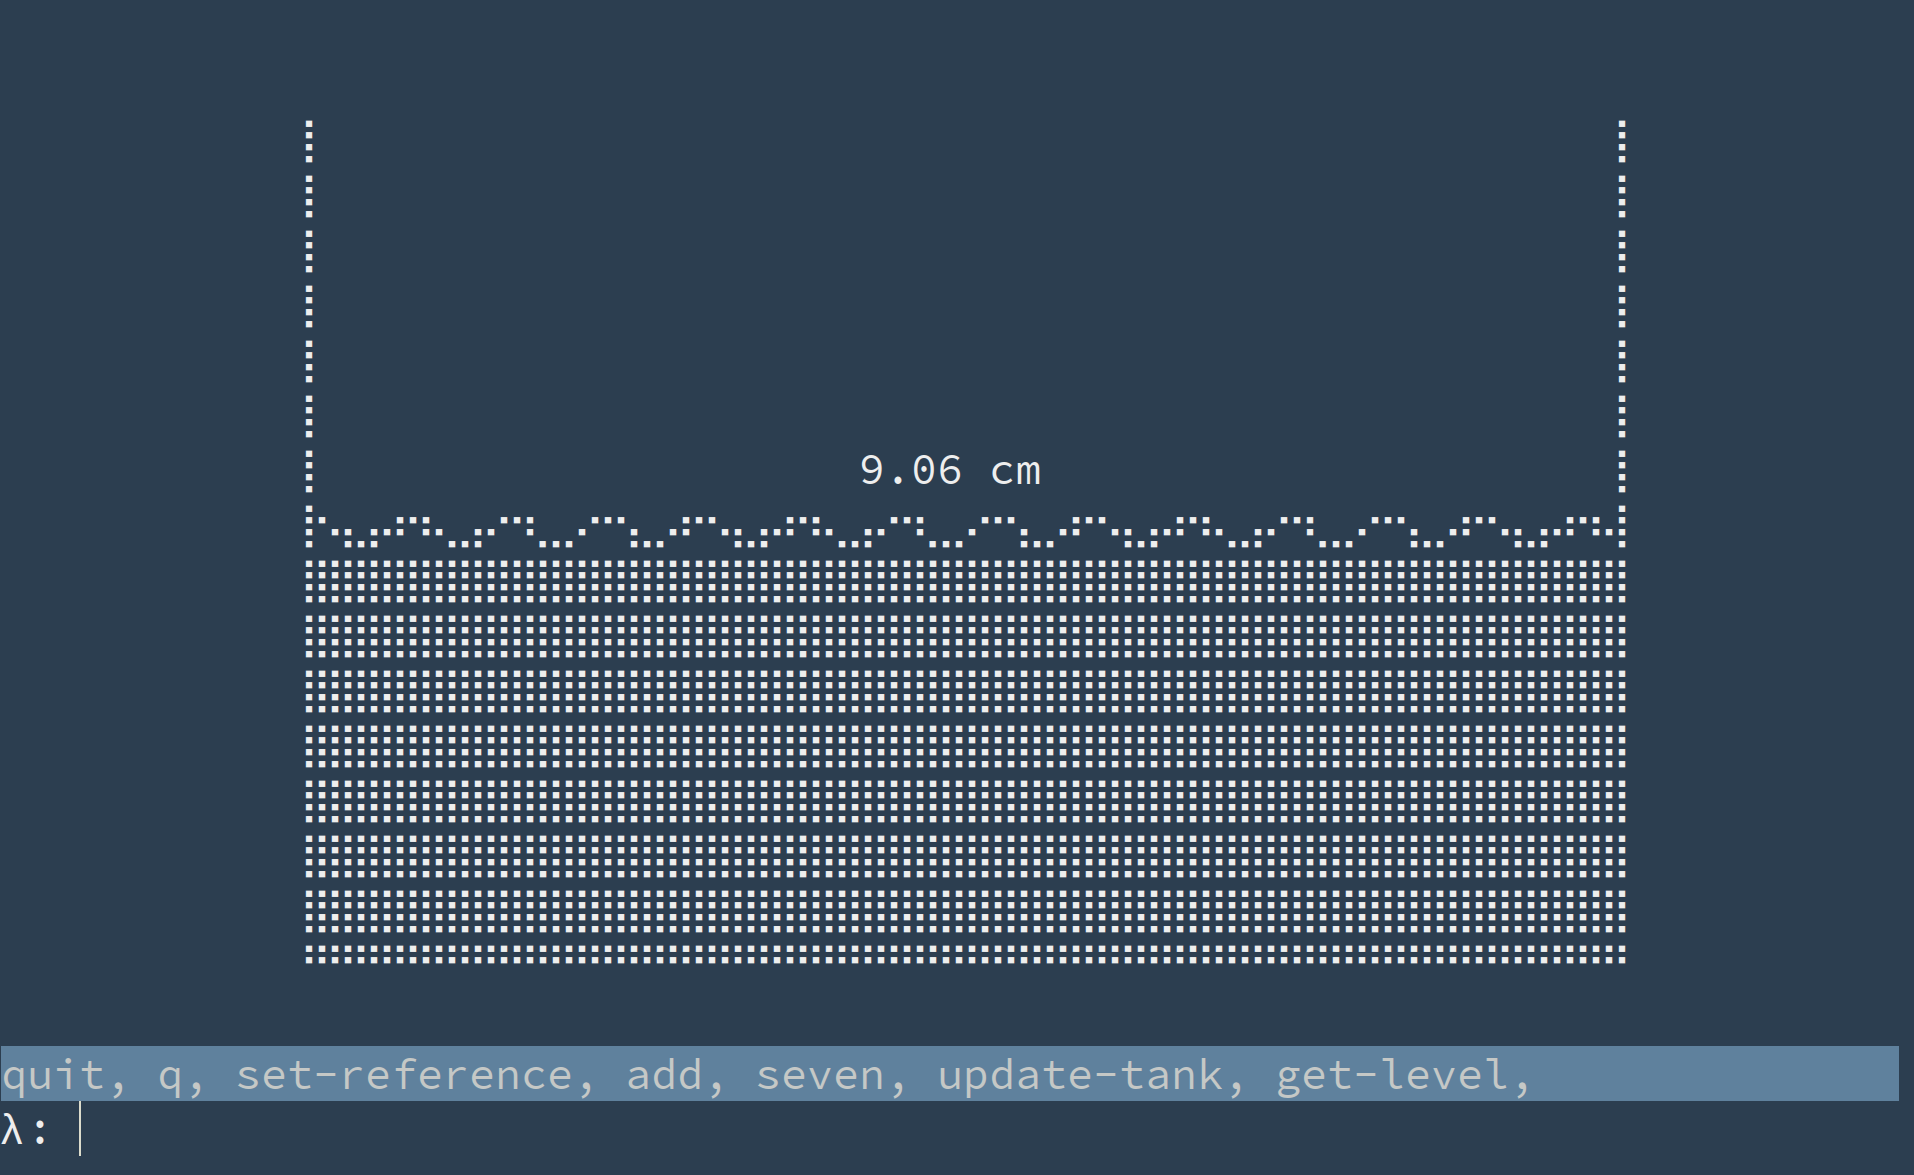
\includegraphics[scale=0.25]{figures/arclient-2.png}
\caption{Prikaz klijenta}
\label{fig:client}
\end{figure}

Na slici \ref{fig:client} je prikazano grafičko sučelje klijenta. Gornji dio
grafičkog sučelja prikazuje shematski prikaz spremnika vode i razinu vode u
stvarnom vremenu. Iznad razine vode ispisana je zadnje mjerena razina vode.

Ispod shematskog prikaza spremnika vode nalazi se informacijski dio komandne
linije to jest statusna linija gdje su trenutno ispisane sve podržane naredbe:
\begin{itemize}
    \item quit
    \item q
    \item set-reference
    \item add
    \item seven
    \item update-tank
    \item get-level
\end{itemize}

Naredbe su odvojene u lokalne i udaljene naredbe. Lokalne naredbe su: \emph{quit}
i \emph{q}. Naredba \emph{quit} služi za gašenje klijenta, a naredba \emph{q} je
samo alias na naredbu \emph{quit}.

Udaljene naredbe su: \emph{set-reference}, \emph{add}, \emph{seven},
\emph{update-tank}, \emph{get-level}. Sve udaljene naredbe generiraju JSON-RPC
poziv te ga šalju serveru i registriraju funkcije koje će obraditi odgovor kad
on stigne.

Naredba \emph{set-reference} je najvažnija naredba klijenta, ona nam omogućuje
promjenu referentne vrijednosti u stvarnom vremenu. Kao argument prima razinu
vode u boci te ga spremi u JSON-RPC poziv. Ukoliko dolazi do greške, greška se
ispisuje u statusnoj liniji.

Naredba \emph{add} je testna naredba koja prima dva brojčana argumenta te ih
serveru u JSON-RPC pozivu šalje. Server će zbrojiti primljene brojčane argumente
i rezultat zbrajanja poslati natrag u JSON-RPC odgovoru. Nakon što odgovor
stigne njegov rezultat bit će prikazan u statusnoj liniji.

Naredba \emph{seven} je također testna naredba, ona šalje serveru unutar
JSON-RPC poziva broj sedam. Server u JSON-RPC odgovoru šalje istu brojčanu
vrijednost natrag. Naredba služi kao jednostavni \emph{echo} test. Rezultat
odgovora se prikazuje u statusnoj liniji.

\emph{update-tank} naredba je naredba koja se izvršava automatski kao dio
periodičkih zadataka koje event loop obavlja. Naredba dohvaća trenutnu razinu
postrojenja te ga prosljeđuje \mintinline{py3}{TankWidget} grafičkom elementu
koji osvježava iscrtavanje shematskog prikaza ukoliko je došlo do promjene.
\emph{get-level} naredba šalje isti JSON-RPC poziv kao i \emph{update-tank}
naredba no umjesto da trenutnu razinu prosljedi grafičkom elementu za prikaz ona
razinu jednostavno prikaže u statusnoj liniji.

Ispod statusne linije nalazi se sama komandna linija u koju je moguće prije
navedene naredbe upisati.

\newpage
\section{Postrojenje}

Postrojenje je napravljeno u obliku makete spremnika u kojem se održava razina
vode. Ulazni tok u spremnik je ostvaren pomoću vodene pumpe kojoj se brzinom
može upravljati pomoću pulsno širinske modulacije. Izlazni tok spremnika je
ostvaren pomoću otvora pri dnu spremnika te voda slobodnim padom teće iz
spremnika. Razina u spremniku se direktno mjeri pomoću senzora.

\begin{figure}[H]
\centering
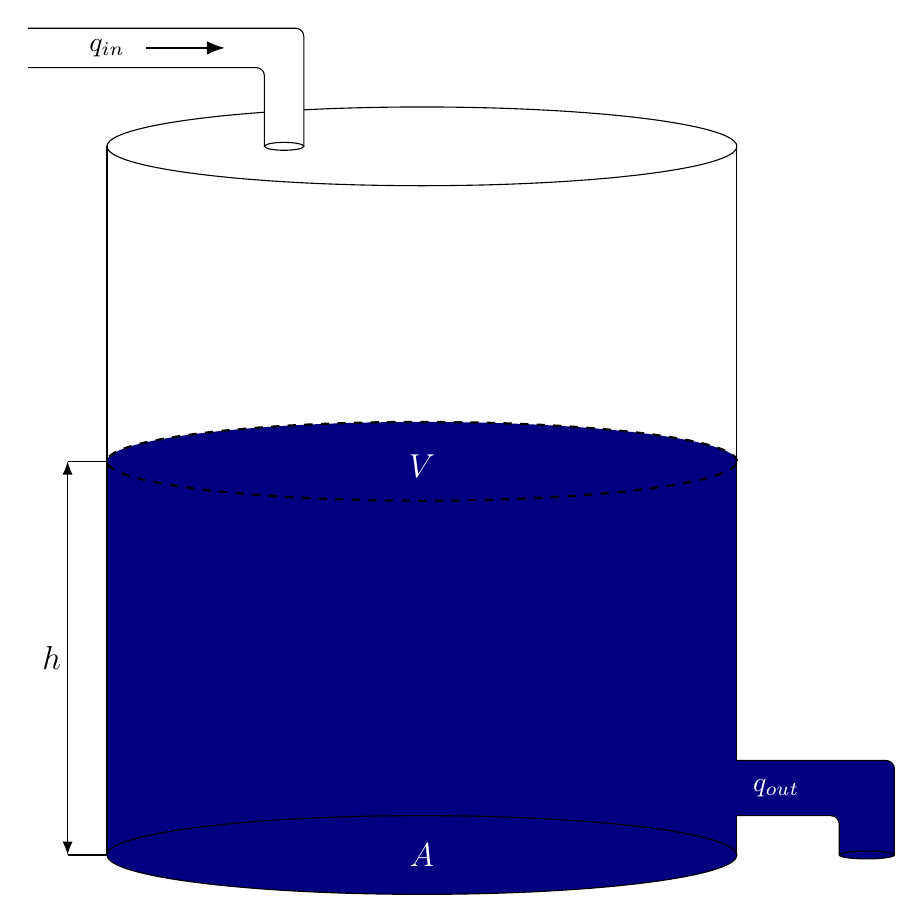
\begin{tikzpicture}[every node/.style = {font = \footnotesize}]
    \tikzset{weird fill/.style={append after command={
    \pgfextra
        \draw [#1, sharp corners, fill=#1]%
        (\tikzlastnode.west)%
        [rounded corners=0] |- (\tikzlastnode.north)%
        [rounded corners=3] -| (\tikzlastnode.east)%
        [rounded corners=0] |- (\tikzlastnode.south)%
        [rounded corners=0] -| (\tikzlastnode.west);
        \endpgfextra}}}

    \draw [rounded corners=3] (-5,10) -- (-2,10) -- (-2,9);
    \draw [rounded corners=3] (-5,10.5) -- (-1.5,10.5) -- (-1.5,9);
    \draw (-1.75, 9) circle [x radius=0.25, y radius=0.05];
    \draw (-4, 10.25) node [font=\normalsize] {$q_{in}$};
    \draw [-Latex, thick] (-3.5, 10.25) -- (-2.5, 10.25);

    \draw (0, 2.5) node[rectangle, minimum width=228, minimum height=140,
    fill=NavyBlue] {};

    \draw [fill=NavyBlue] (0,0) circle [x radius=4, y radius=0.5];
    \draw [fill=NavyBlue, thick, dashed] (0,5) circle [x radius=4, y radius=0.5];

    \node [font=\large] (area) {\textcolor{white}{$A$}};
    \node [font=\large, above=4.4 of area] {\textcolor{white}{$V$}};

    \draw (4,9)  arc[x radius = 4, y radius = 0.5, start angle=0, end angle=112];
    \draw (4,9)  arc[x radius = 4, y radius = 0.5, start angle=0, end angle=-240];

    \draw (-4,0)  -- (-4,9);
    \draw (4,0)   -- (4,0.5);
    \draw (4,1.2) -- (4,9);

    \draw (4.9, 0.85)
    node[weird fill=NavyBlue, rectangle, minimum width=62, minimum height=19]
    (qout1) {};
    \draw (4.5, 0.85) node [font=\normalsize] {\textcolor{white}{$q_{out}$}};

    \node [below right=-0.1 and -0.7 of qout1, fill=NavyBlue, minimum width=20, minimum
    height=17] (qout2) {};

    \draw [NavyBlue, fill=NavyBlue] (5.2, 0.6) -- (5.2,0.7) -- (5.5,0.7) -- (5.30, 0.4);
    \draw [NavyBlue, fill=NavyBlue] (5.2, 0.6) -- (5.2,0.5) -- (5.5,0.49);
    \draw [rounded corners=3] (4,1.2) -- (6,1.2) -- (6,0);
    \draw [rounded corners=3] (4,0.5) -- (5.3,0.5) -- (5.3,0);

    \draw [fill=NavyBlue] (5.65,0) circle [x radius=0.35, y radius=0.05];

    \draw (-4, 0) -- (-4.5, 0);
    \draw (-4, 5) -- (-4.5, 5);
    \draw [Latex-Latex] (-4.5, 0) -- (-4.5, 5);
    \draw (-4.7, 2.5) node [font=\large] {$h$};

\end{tikzpicture}
\caption{Shematski model postrojenja}
\label{fig:plant}
\end{figure}

Na slici \ref{fig:plant} se vidi postrojenje. Iznad glavnog spremnika se vidi
ulazna cijev sa ulaznim tokom $q_{in}$ dok se u desnom dijelu glavnog spremnika
nalazi otvor za izlazni tok $q_{out}$.

Razina vode u spremniku označena je sa $h$ dok je volumen koji voda zauzima u
spremniku označen sa $V$. Površina poprečnog presjeka spremnika je označena sa
$A$.

\newpage
\subsection{Matematički model postrojenja}


Volumen vode u spremniku ovisi o ulaznom toku i izlaznom toku. Volumen će ostat
konstantan ukoliko su ulazni i izlazni tok isti dok će se volumen vode mijenjati
ovisno o razlici ulaznog toka i izlaznog toka, s toga možemo reći:

\begin{equation}
    \frac{dV}{dt} = q_{in} - q_{out}
\label{eq:first}
\end{equation}

Gdje je ulazni tok definiran kao:

\begin{equation} q_{in} = k_p U \end{equation}

gdje je:
\begin{description}[labelindent=2cm]
        \item[$k_p$] - konstanta pumpe
        \item[$U$]   - napon pumpe
\end{description}

Izlazni tok je određen pomoću Torricellijevog zakona \cite[75]{fluid}:

\begin{equation} q_{out} = a \sqrt{2gh} \end{equation}

gdje je:
\begin{description}[labelindent=2cm]
        \item[$a$] - poprečni presjek izlazne cijevi
        \item[$g$] - ubrzanje zemljine sile teže
            (\unit{9.80665}{\metre\per\square\second})
        \item[$h$] - visinska razina vode u spremniku
\end{description}

Pošto je spremnik cilindričnog oblika možemo za volumen spremnika vrijedi
jednakost $V = A h$. Uvrštavanjem ulaznog i izlaznog toka te jednakosti za
volumen u jednadžbu \ref{eq:first} dobiva se:

\begin{equation}
    A\frac{dh}{dt} = k_p U - a \sqrt{2gh}
\label{eq:nonlin}
\end{equation}

Iz jednadžbe \ref{eq:nonlin} se vidi da ona sadržava nelinearni element u obliku
$a \sqrt{2gh}$, da bi uspješno mogli analizirati sustav i primjeniti Laplaceovu
transformaciju jednadžba koja opisuje sustav mora biti linearizirana
\cite[88-97]{control}:

\begin{equation} \frac{d\delta h}{dt} = \frac{k_p}{A} \delta U -
                 \frac{a \sqrt{2g}}{2 A \sqrt{h_0}} \delta h \end{equation}

gdje je:
\begin{description}[labelindent=2cm]
        \item[$h_0$] - radna točka oko koje je sustav lineariziran
\end{description}

Konstantne vrijednosti uz $\delta U$ i $\delta h$ se radi jednostavnosti mogu
staviti u poseban izraz:

\begin{equation}
    \frac{d\delta h}{dt} = k_1 \delta U - k_2 \delta h
\end{equation}

Sada se može primjeniti Laplaceova transformacija \cite[35-44]{control} pri čemu
dobiva se:
\begin{equation} s H(s) = k_1 U(s) - k_2 H(s) \end{equation}

Nakon grupiranja $H(s)$ elemenata na lijevoj strani jednadžbe dobiva se:
\begin{equation} H(s)(s+k_2) = k_1 U(s) \end{equation}

Te konačno se dobiva prijenosna funkcija sustava \cite[45]{control}:
\begin{equation}
    G(s) = \frac{H(s)}{U(s)} = \frac{k_1}{s+k_2}
\label{eq:transfer}
\end{equation}

Iz jednadžbe \ref{eq:transfer} se vidi da jednadžba predstavlja sustav prvog
reda \cite[166]{control}. Osim što je sustav poprilično jednostavan on je i samo
stabilizirajući \cite{control_guru} tj. za svaku ulaznu veličinu sustav će se
nakon određenog vremena stabilizirati.

Zbog jednostavnosti sustava možemo odabrati jednostavni PI regulator koji će
omogućiti brz dolazak u stacionarno stanje te smanjiti regulacijsku grešku
stacionarnog stanja.

\subsection{Senzor i aktuator}

Da bi regulator mogao obavljati svoj posao mora imati uvid u stanje sustava te
mora imat način na koji promjeniti stanje. Uvid u stanje regulatoru pruža senzor
razine tekućine a promjena stanja je moguća pomoću pumpe tekućine.

Za senzor je korišten \emph{eTape} senzor razine tekućine \cite{etape}. Senzor
je realiziran kao promjenjivi otpornik čiji se otpor mijenja ovisno na kojem
dijelu senzora hidostatski tlak tekućine pritišće senzora. Izlazni otpor senzora
je inverzno proporcionalan sa razinom tekućine.

Radi veće preciznosti mjerenja izlazni otpor senzora pretvara se u napon raspona
od \unit{0-5}{\volt}. Pretvorba izlaznog otpora u napon je ostvarena pomoću
\emph{\unit{0-5}{\volt} Linear Resistance to Voltage Module} istog proizvođača
kao i senzor \cite{voltage_module}.

\begin{table}[h]
\setlength{\tabcolsep}{14pt}
\centering
    \begin{tabular}{|c|c|c|c|c|c|c|c|}
        \hline
        Napon (\volt) &
        0.36  &  0.56  &  0.78  & 1.01  & 1.19  & 1.40 &  1.66 \\
        \hline
        Razina vode (\centi\metre) &
        4  &  5  &  6  &  7  &  8  &  9  & 10 \\
        \hline
        \hline
        Napon (\volt) &
        1.85  &  2.05  &  2.25  & 2.53  & 2.83  & 2.97 &  3.26 \\
        \hline
        Razina vode (\centi\metre) &
        11  & 12  & 13 &  14 &  15&16 &  17 \\
        \hline
    \end{tabular}
    \caption{Kalibracijske vrijednosti senzora}
    \label{tbl:etape}
\end{table}

U tablici \ref{tbl:etape} se vide mjerene naponske vrijednosti senzora uz
određene razine vode. Senzor ima mrtvi pojas od \unit{0-2.54}{\centi\metre} u
kojem se otpor te u konačnici napon ne mijenjaju.

\begin{figure}[H]
\centering
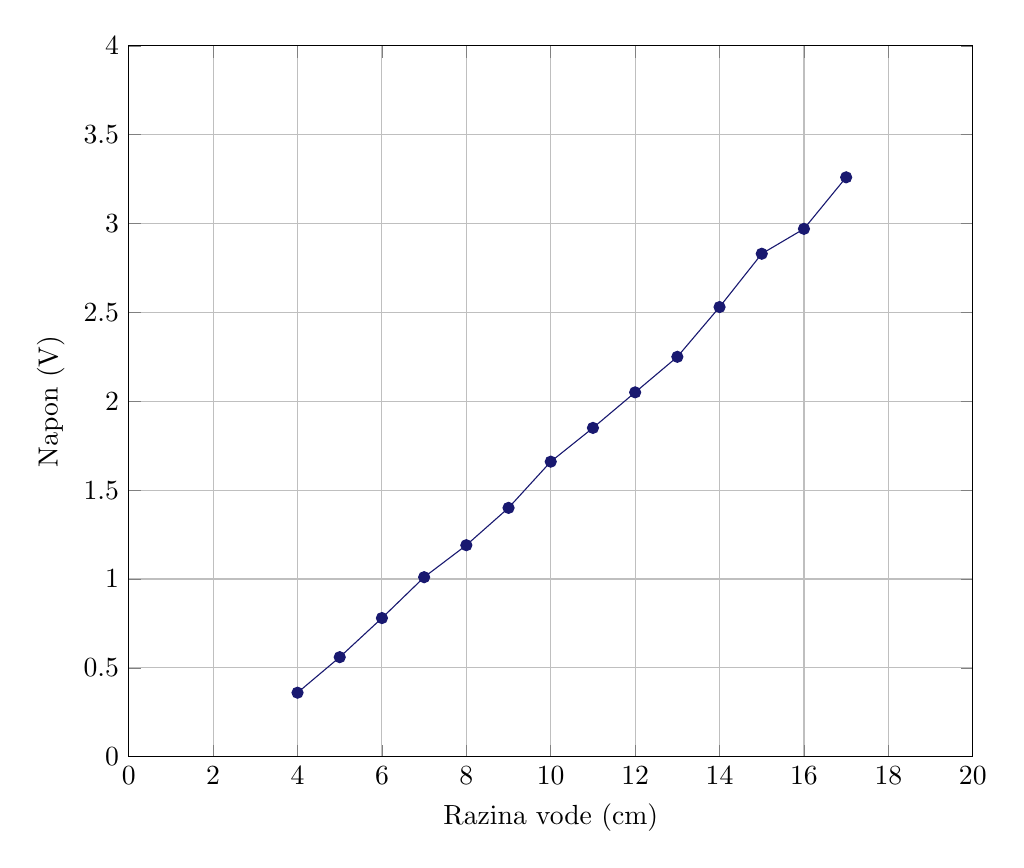
\begin{tikzpicture}
    \begin{axis}[width=350, xlabel=Razina vode (\centi\metre), ylabel=Napon
                 (\volt), grid=major, ymin=0, ymax=4, xmin=0, xmax=20]
    \addplot[color=MidnightBlue, mark=*] coordinates {
        (4, 0.36)
        (5, 0.56)
        (6, 0.78)
        (7, 1.01)
        (8, 1.19)
        (9, 1.4)
        (10, 1.66)
        (11, 1.85)
        (12, 2.05)
        (13, 2.25)
        (14, 2.53)
        (15, 2.83)
        (16, 2.97)
        (17, 3.26)
    };
    \end{axis}
\end{tikzpicture}
\caption{Graf odziva senzora}
\label{fig:etape}
\end{figure}

Na grafu \ref{fig:etape} se vidi promjena napona ovisno o razini vode. Jasno je
vidljiv linearni odziv senzora.

Pumpa koja je odabrana je mala pumpa za modelske svrhe maksimalnog protoka od
\unit{1.84}{\litre\per\minute}. Protok pumpe se može regulirati naponski.
Minimalni napon pumpe je \unit{3}{\volt}, a maksimalni \unit{12}{\volt}.

\begin{table}[h]
\setlength{\tabcolsep}{14pt}
\centering
    \begin{tabular}{|c|c|c|c|c|c|c|}
        \hline
        Napon (\volt) & 12 & 10 & 8 & 5 & 4 & 3 \\
        \hline
        Protok (\centi\cubic\metre\per\second) &
        28.8889 & 23.3332 & 18.4193 & 11.3328 & 8.1663 & 5.0008 \\
        \hline
    \end{tabular}
    \caption{Kalibracijske vrijednosti pumpe}
    \label{tbl:pump}
\end{table}

U tablici \ref{tbl:etape} se vidi mjereni protok pumpe senzora uz
određene naponske razine.

\begin{figure}[H]
\centering
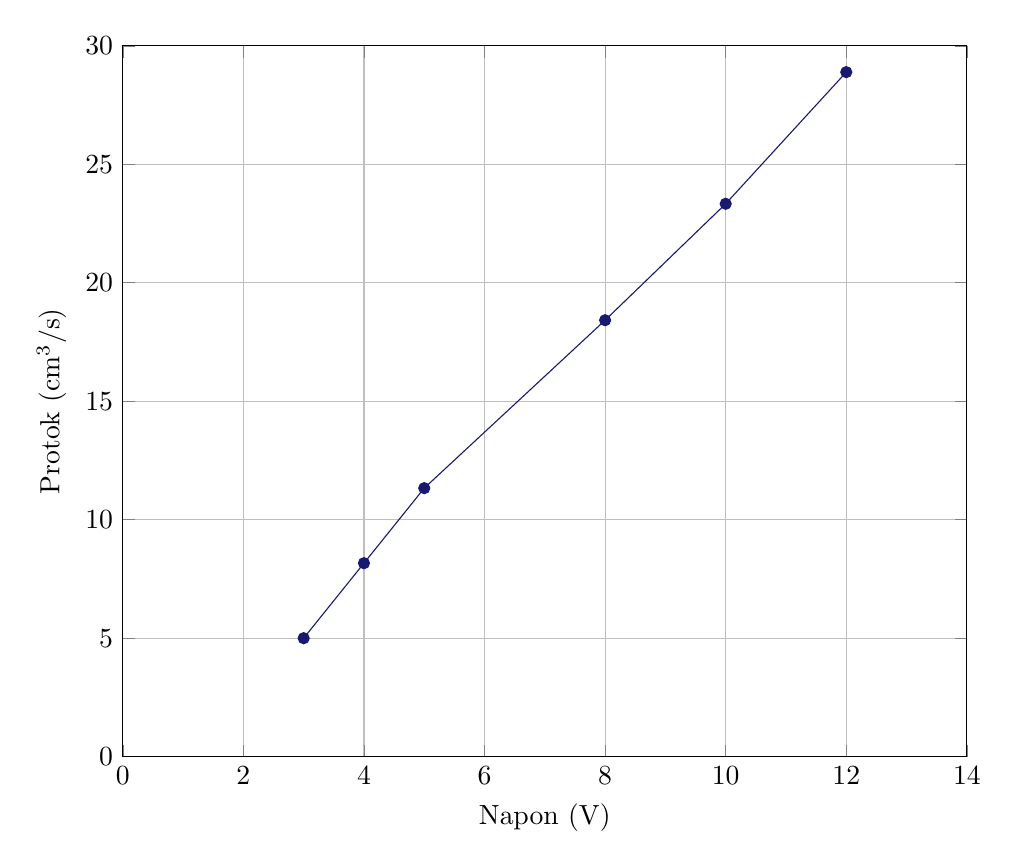
\begin{tikzpicture}
    \begin{axis}[width=350, xlabel=Napon (\volt), ylabel=Protok
                 (\centi\cubic\metre\per\second), grid=major, xmin=0, xmax=14,
                 ymin=0, ymax=30]
    \addplot[scale=2, color=MidnightBlue, mark=*] coordinates {
        (3, 5.0008)
        (4, 8.1663)
        (5, 11.3328)
        (8, 18.4193)
        (10, 23.3332)
        (12, 28.8889)
    };
    \end{axis}
\end{tikzpicture}
\caption{Graf odziva pumpe}
\label{fig:pump}
\end{figure}

Na grafu \ref{fig:pump} se vidi promjena protoka pumpe ovisno o naponskoj
razini. Zbog ograničenog maksimalnog protoka pumpe brzina odziva sustava ovisi o
veličini spremnika. Za relativno brz odziv sustava je odabrana boca volumena od
\unit{1}{\litre}. Boca je cilindričnog oblika radius joj je
\unit{4}{\centi\metre}, a visina nešto ispod \unit{20}{\centi\metre}. Zbog
mrtvog pojasa senzora regulacija ispod \unit{3}{\centi\metre} nije moguća.

\newpage
\subsection{Arduino shield}

Operativni napon izlazno/ulaznih pinova Arduino mikroupravljačke pločice je u
rasponu od \unit{0-5}{\volt} te nije u stanju iskoristiti čitav operativni
raspon pumpe. Da bi se mogao iskoristiti čitav operativni raspon pumpe koristi
se \emph{L293E} integrirani krug za pogon istosmjernih motora \cite{h-bridge}.

\begin{figure}[H]
\centering
\includegraphics[scale=0.80]{figures/shield_schematic.pdf}
\caption{Električna shema postrojenja}
\label{fig:schematic}
\end{figure}

Slika \ref{fig:schematic} prikazuje potpunu električnu shemu postrojenja gdje
je:
\begin{description}[labelindent=2cm]
        \item[IC1] - Arduino mikroupravljačka pločica
        \item[IC2] - L293E IC za pogon istosmjernih motora
        \item[IC3] - Modul koji pretvara otpor senzora u napon
        \item[S]   - \emph{eTape} senzor razine tekućine
        \item[P]   - \unit{12}{\volt} pumpa
        \item[D1]  - zaštitna dioda
        \item[C1]  - stabilizacijski kondenzator
\end{description}

Shema također prikazuje spojeve između svih komponenti postrojenja. Analogni
ulaz Arduina A0 je spojen na izlaz IC3 modula. Arduino na analognom ulazu A0
prima \unit{0-5}{\volt} signal koji je proporcionalan sa razinom vode. Na
\emph{L293E} integriranom krugu su pinovi za pogon prvog i četvrtog kanala
kratkospojeni te se opterećenje tjekom rada raspodjeljuje na oba kanala.

Digitalni pin D2 koji je konfiguriran kao izlaz je spojen na \emph{Chip Enable}
pin \emph{L293E} integriranog kruga, s njime se upravlja aktivaciju pogonskih
kanala integriranog kruga. Napon na izlazu \emph{L293E} integriranog kruga ovisi
o naponu na ulazu, ulaznim naponom upravljamo pomoću izlaznog pina D3 na
Arduinu.

D3 pin Arduina je konfiguriran kao pulsno širinski izlazni pin. Izlazni
pin \emph{L293E} integriranog kruga je spojen na pumpu. Paralelno s pumpom je u
spoju dioda D1, ona štiti strujni krug od induktivnog napona koji se pojavljuje
pri gašenju pumpe.

\subsection{Regulator}

Regulator koji je dio servera komunicira s Arduinom te pomoću Arduina upravlja s
postrojenjem. Osnovna zadaća mu je primiti željenu referentnu vrijednost te
sustav dovesti u novo stacionarno stanje i držati ga tamo.

Radi jednostavnosti i niskog reda sustava za regulator je odabran PI
regulacijski algoritam.

\begin{listing}[H]
\centering
\begin{minted}[frame=single]{haskell}
forever $ do
    reference <- liftIO $ readMVar refMVar
    integral  <- liftIO $ takeMVar integralMVar

    sensorValue <- analogRead sensor
    let fillHeight = sensorValueFunc sensorValue
    _ <- liftIO $ swapMVar pvMVar fillHeight
    let error = reference - fillHeight

    let proportional_term = kp * error
    let integral_term     = integral + ki * error / sampleTime
    liftIO $ putMVar integralMVar integral_term

    let output = clampAndScaleOutput $ proportional_term + integral_term

    analogWrite pwm_pin output
    delay sampleTime
\end{minted}
\caption{Regulacijska petlja}
\label{lst:regulator}
\end{listing}

Na ispisu koda \ref{lst:regulator} je prikazana regulacijska funkcija koja se
nalazi unutar servera. Prvo se uzima referenca i vrijednost integratora iz dijeljenih varijabli.
\mintinline{haskell}{integralMVar} je interna varijabla regulatora gdje se
sprema akumulirana vrijednost integratora dok je \mintinline{haskell}{refMVar}
dijeljena varijabla u koju posrednička funkcija stavlja referentnu vrijednost.

Odmah nakon čitanja dijeljenih varijabli zatražuje se od Arduina trenutna
razina vode pomoću \mintinline{haskell}{analogRead} funkcije. Razina se pretvara
iz naponske vrijednosti u visinu pomoću \mintinline{haskell}{sensorValueFunc} te
se sprema u \mintinline{haskell}{fillHeight} varijablu i prosljeđuje ostatku
servera spremajući je u za to namjenjenu dijeljenu varijablu.

Nakon što je mjerenje izvršeno i preuzeta je trenutna referentna vrijednost,
pomoću istih se računa odstupanje od referentne vrijednosti te se sprema u
\mintinline{haskell}{error} varijablu. Integralni dio regulatora se sprema u
prije spomenutu varijablu \mintinline{haskell}{integralMVar} koja će je
sačuvati za sljedeću iteraciju regulacijske petlje.

Sada se mogu proporcionalni i integralni članovi regulatora izračunati te
zbrojiti. Funkcija \mintinline{haskell}{clampAndScaleOutput} ograničava izlaz
regulatora na operativni raspon pumpe, brine se o tome da pumpa ne pokušava
raditi na naponu ispod \unit{3}{\volt}.

Preostaje samo poslati novu naponsku razinu na Arduinu te će ju on primjeniti na
pulsno širinskom pinu i tako postaviti protok pumpe. Nakon toga petlja čeka
određeno vrijeme te ponovno izvršava sve navedene korake.

\begin{figure}[H]
\centering
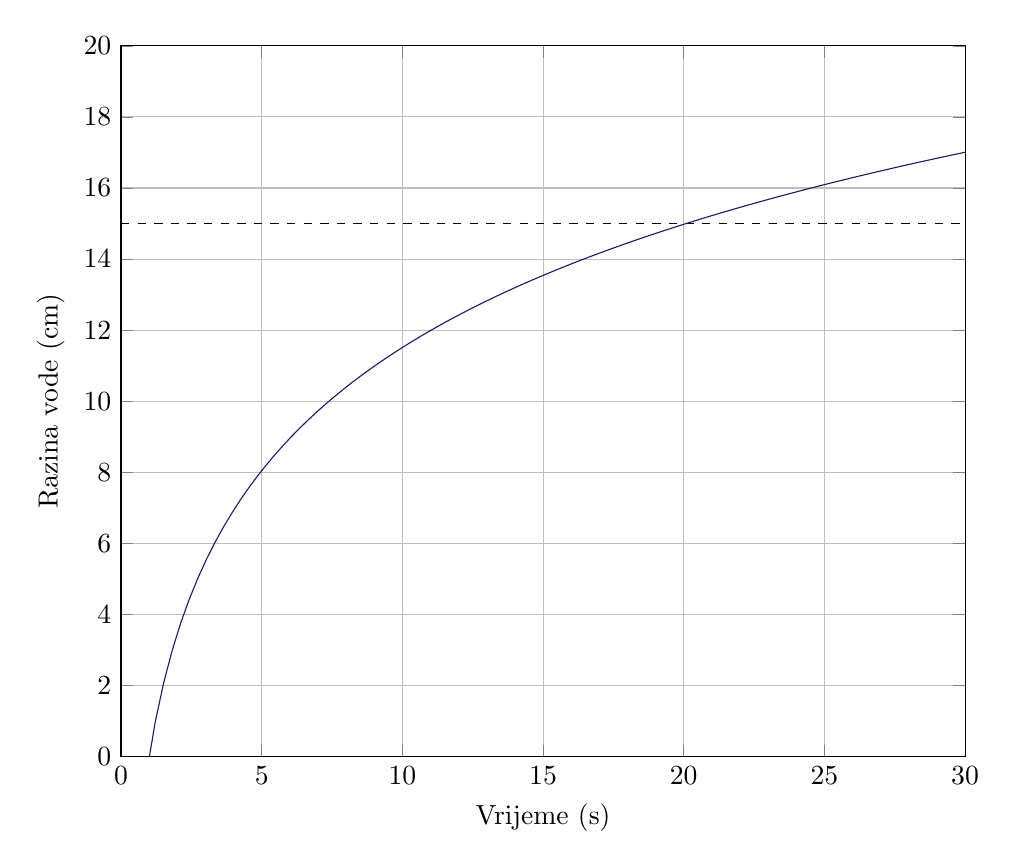
\begin{tikzpicture}
    \begin{axis}[width=350, xlabel=Vrijeme (\second), ylabel=Razina vode
                 (\centi\metre), grid=major, xmin=0, xmax=30,
                 ymin=0, ymax=20]
                 \addplot[samples=100, domain=0:30, dashed] { 15 };
%                 \addplot table [x=a, y=c, col sep=comma] {data.csv};
                 \addplot[scale=2, color=MidnightBlue, samples=100, domain=0:30] {
                    ln(x) * 5
                 };
    \end{axis}
\end{tikzpicture}
\caption{Graf odziva regulatora}
\label{fig:step_response}
\end{figure}

Na slici \ref{fig:step_response} je prikazan odziv regulatora uz $k_p = 4$ i
$k_i = 1.5$.

\newpage
\chapter{Zaključak}

U radu je razvijen i predstavljen socket server za komunikaciju s postrojenjem.
Server komunicira s Arduino mikroupravljačkom pločicom i upravlja postrojenjem
koje je spojeno na pločicu. Demonstrirano je uspješno automatsko upravljanje
razine vode u spremniku. Razvijen je i klijent koji u stvarnom vremenu daje uvid
u stanje postrojenja te omogućuje udaljenu promjenu regulirane veličine. Tijekom
izrade, glavni problemi bili su omogućavanje istovremenog obavljanja poslova
regulacije i posluživanja podataka udaljenim klijentima, izrada makete
postrojenja te povezivanje svih dijelova rada u cjelinu.

Predstavljeno riješenje koje koristi regulator unutar socket servera ima svoje
prednosti i nedostatke. Nedostatci su vezani uz brzinu regulacije, zbog
serijskog protokola koji je korišten za komunikaciju postrojenja i socket
servera nije moguće regulirati procese koji imaju jako ograničene vremenske
zahtjeve. Zahtjev za dodatnim računalom pored mikroupravljača za obavljanje
posla regulacije također je jedan nedostatak. Prednosti su mogućnost rapidnog
razvoja regulatora, mogućnost izmjene regulatora bez ponovnog programiranja
mikroupravljača, mogućnost udaljenog upravljanja postrojenjem te fleksibilnost.

Široka dostupnost jeftinih mikroupravljača te malih računalnih platformi
omogućuje korištenje predstavljenog rješenja u razne svrhe kućne
automatizacije. Moguća je izrada mreže automatizirnih procesa kojima je
omogućeno daljinsko upravljanje pomoću socket servera.

Riješenje također ima visoki potencijal za poboljšanja. Moguće je poboljšati
parametre regulatora te ostvariti bolje upravljanje, prebaciti regulator na
mikroupravljač te tako smanjiti latenciju. Na serveru se lako mogu
implementirati razne vrste regulatora te bi se one mogle dinamički izmjenjivati.
Komunikacija klijenta i servera izvršava se nekriptiran. Na serveru
se također može implementirati zahtjev za autentikacijom prije nego se dozvoli uvid u
stanje postrojenja.


% No page numbers from here on.
\renewcommand{\thepage}{}

\printbibliography[heading=bibintoc, title=Literatura]

\newpage

\chapter*{Sažetak}
\addcontentsline{toc}{chapter}{Sažetak}
Pojavom jeftinih mikroupravljača i mini računala mogućnosti povezivanja
fizikalnog svijeta s digitalnim postaju sve veće.
Svrha diplomskog rada je ispitivanje mogućnost korištenja jeftinih mikroupravljača
za jednostavne poslove automatizacije kao i udaljenog upravljanja postrojenja 
preko \emph{socket} \emph{servera}.

Za mikroupravljač \emph{Arduino Uno} preko USB-serijskog sučelja i preko \emph{Firmata} 
protokola komunicira s računalom. Na njega je je vodena pumpa i senzor koji mjeri 
razinu vode u boci te sustav od dvije boce. Na računalu se nalazi \emph{socket} \emph{server} 
pisan u \emph{Haskellu} koji upravlja mikroupravljačem. Testni klijent pisan u 
\emph{Pythonu} spaja se na \emph{server} te dohvaća mjernu veličinu 
i prikazuje trenutno stanje sustava.

Rad je podijeljen u dva dijela: teorijski dio koji detaljno opisuje proces razvoja socket 
servera te praktični dio koji se bavi implementacijom postrojenja, regulatora, \
emph{socket servera} i popratnog klijenta.
\\

\noindent\textbf{Ključne riječi:} Haskell, Arduino, Automatizacija,
Python, Socket server, Firmata
\chapter*{Abstract}
The rise of cheap microcontrollers and mini computers have enabled new possibilities
of connecting the physical world with the digital.
The purpose of this paper is to explore the possibilities of cheap microcontrollers 
for simple automation as well as to enable remote control using a socket server.

The microcontroller Arduino Uno was chosen which communicates through the USB 
interface and the  Firmata protocol with the computer. A water pump and a sensor, 
which measures the water level, were connected as well as two bottles. 
The computer is equipped with a socket server written in Haskell 
which controls the microcontroller. The test client written in Python is being 
connected to the server and pumps the requested amount of water and shows the 
current system status.

The paper is divided into two parts. The first part shall elaborate the theoretical presuppositions 
regarding the subject matter. The second shall address the implementation of the system, 
the regulators, the socket servera and the accompanying client.
\\

\noindent\textbf{Keywords} Haskell, Arduino, Automation,
Python, Socket server, Firmata

\newpage

\chapter*{Životopis}
\addcontentsline{toc}{chapter}{Životopis}

Damir Jelić rođen je 8.~ožujka 1989.~godine u Osijeku. Osnovno
obrazovanje stekao je u osnovnoj školi Šećerana u Šećerani. Nakon toga,
pohađao je Prvu srednju školu u Belom Manastiru, smjer Tehničar računarstva,
2007. godine polaže maturu i iste godine upisuje Preddiplomski studij
Računarstva na Elektrotehničkom fakultetu u Osijeku. 2010. godine završava
Preddiplomski studij računarstva te upisuje Diplomski studij Procesnog
računarstva. Dva puta je sudjelovao u programu Google Summer of Code: oba puta u
sklopu PulseAudio organizacije, gdje je radio na dinamičkom podešavanju latencije
i \emph{resampling} poboljšanjima za PulseAudio softverski projekt.

\vspace{1cm}
\noindent \vspace*{1.0cm} \makebox[1.5in]{\hrulefill}

\chapter*{Prilozi}
\addcontentsline{toc}{chapter}{Prilozi}

\section*{Prikaz spremnika sa senzorom}

\begin{figure}[h]
\centering
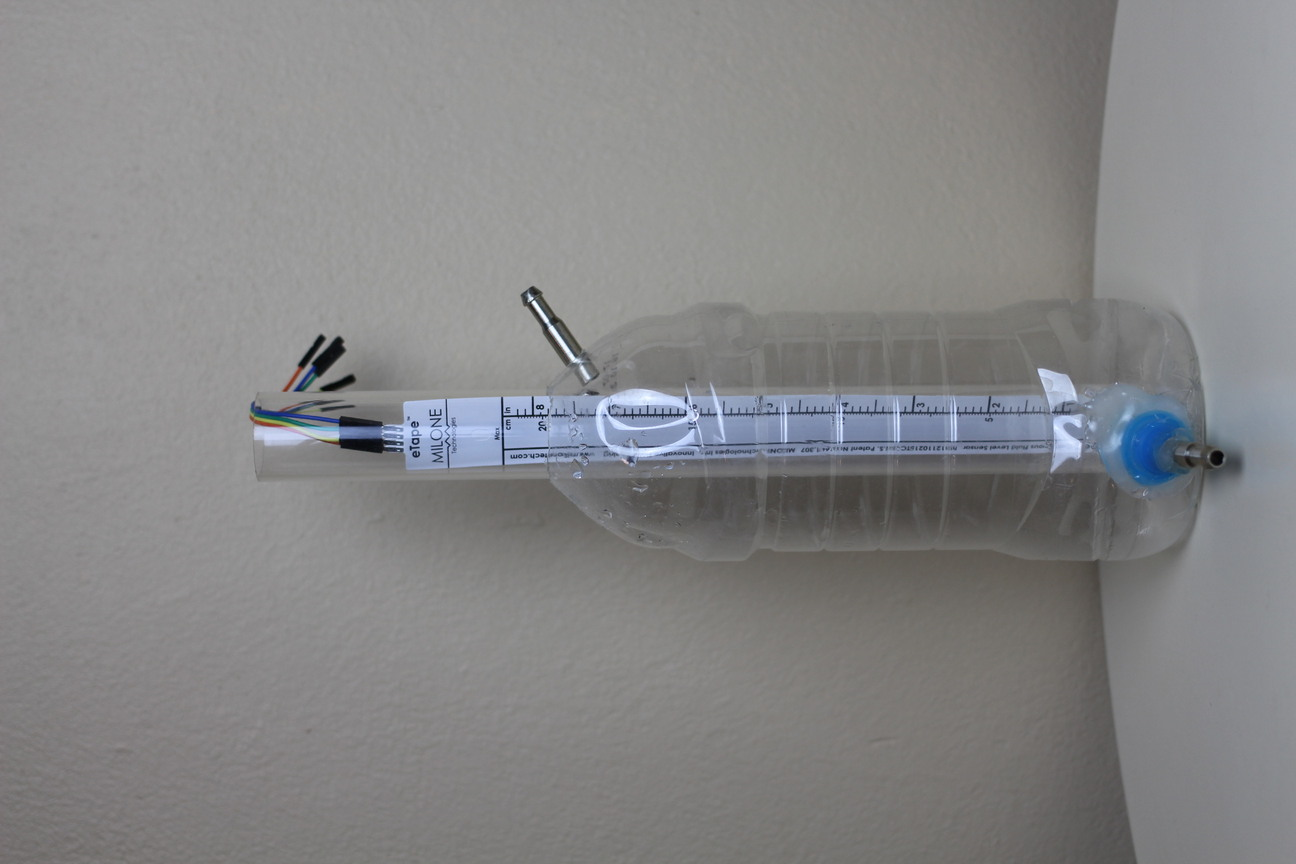
\includegraphics[angle=-90, scale=0.4]{figures/tank_picture_resized.jpeg}
\end{figure}

\newpage
\section*{Prikaz Arduina i popratnog \emph{shielda}}

\begin{figure}[h]
\centering
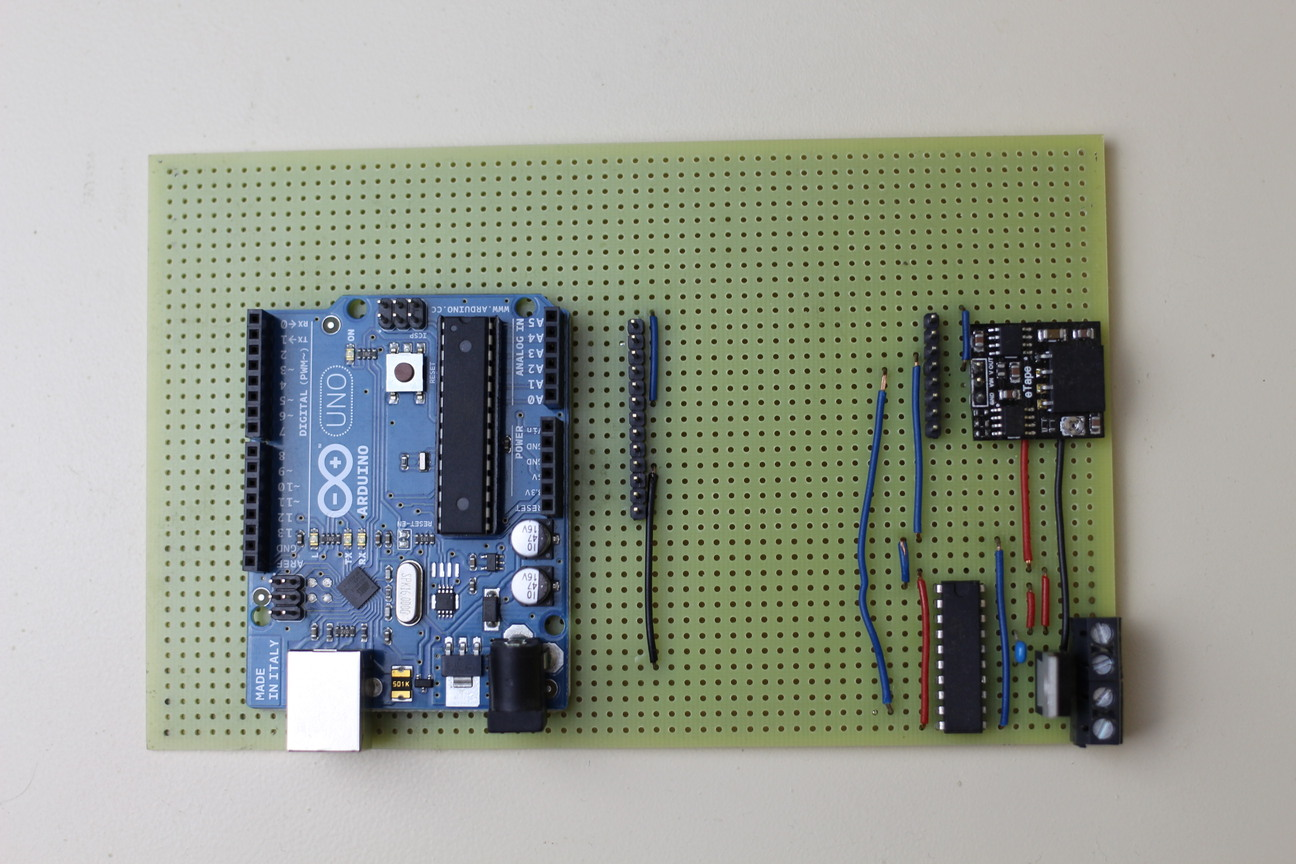
\includegraphics[angle=90, scale=0.4]{figures/shield_picture_resized.jpeg}
\end{figure}


\end{document}
